\subsection{柔软层}

定义 5. --- 设 \(p\colon E \rightarrow B\) 为平展映射。称映射 \(p\) 是柔软的，或称平展 B-空间 \((E,p)\) 是柔软的，如果 \(p\) 在 B 的闭子空间上的每个连续截面都能扩张为 \(p\) 在 B 上的一个连续截面。

设 F 为 B 上的一个层。若相伴的平展空间 (I, p. 50, def. 4) 是柔软的，则称 F 为柔软层。

设 \(\mathcal{F}\) 为 B 上的层。层 \(\mathcal{F}\) 是柔软的，当且仅当：对 B 的每个闭集 Z、Z 的每个开邻域 U 以及每个 \(s \in \mathcal{F}(\mathrm{U})\) ，存在 \(t \in \mathcal{F}(\mathrm{B})\) 以及 Z 的一个含于 U 的开邻域 V，使得 \(s \mid \mathrm{V} = t \mid \mathrm{V}\) 。

若 \(\mathcal{F}\) 是柔软层，则 \(\mathcal{F}(\mathrm{B})\) 非空：事实上，平展空间 \(\mathrm{E}_{\mathcal{F}}\) （与层 \(\mathcal{F}\) 相伴者）在 \(\varnothing\) 上的唯一截面可扩张为 \(\mathrm{E}_{\mathcal{F}}\) 在 B 上的连续截面。

设 \(p \colon \mathrm{E} \to \mathrm{B}\) 为平展映射，并设 A 为 B 的闭子空间。若 \(p\) 是柔软的，则映射 \(p_{\mathrm{A}} \colon \overline{p}^{1}(\mathrm{A}) \to \mathrm{A}\) 是柔软的。等价地，若 \(\mathcal{F}\) 是 B 上的柔软层，则它在闭子空间 A 上诱导的层是柔软的。

命题 6. --- 设 B 为拓扑空间，\(\mathcal{F}\) 为 B 上的层，\((\mathrm{A}_i)_{i\in \mathrm{I}}\) 为 B 的局部有限闭覆盖。层 \(\mathcal{F}\) 是柔软的，当且仅当对每个 \(i\in \mathrm{I}\)，诱导层 \(\mathcal{F}_{\mathrm{A}_i}\) 都是柔软的。

该条件显然是必要的。我们来证明它是充分的。用 \(p\colon \mathrm{E}\to \mathrm{B}\) 表示 B-平展空间 \(\mathrm{E}_{\mathcal{F}}\) （与层 \(\mathcal{F}\) 相伴者）。设 A 为 B 的闭子空间，并设 \(s\colon \mathrm{A}\to \mathrm{E}\) 为 \(p\) 在 A 上的一个连续截面；须证 \(s\) 具有到 B 上的连续扩张。对 I 的每个子集 J，令 \(\mathrm{A_J} = \bigcup_{i\in \mathrm{J}}\mathrm{A}_i\) ；集 \(\mathrm{A_J}\) 在 B 中是闭的 (TG, I, p. 6, prop. 4)。

设 \(\mathcal{S}\) 为由数对 \((\mathrm{J},t)\) 组成的集，其中 \(\mathrm{J}\) 是 I 的子集，而 \(t\) 是 E 在 \(\mathrm{A_J}\) 上的连续截面，且与 \(s\) 在 \(\mathrm{A} \cap \mathrm{A_J}\) 上重合。给 \(\mathcal{S}\) 赋以记作 \(\leqslant\) 的序关系：\((\mathrm{J},t) \leqslant (\mathrm{J}',t')\) 如果 \(\mathrm{J} \subset \mathrm{J}'\) 且 \(t' \mid \mathrm{A_J} = t\) 。对 \(\sigma = (\mathrm{J},t) \in \mathcal{S}\) ，记 \(\mathrm{J}_{\sigma} = \mathrm{J}\) 与 \(t_{\sigma} = t\) 。我们来证明序集 \(\mathcal{S}\) 是归纳的。设 S 为 \(\mathcal{S}\) 的一个全序子集。令 \(\mathrm{J} = \bigcup_{\sigma \in \mathrm{S}} \mathrm{J}_{\sigma}\) ；它是 I 的一个子集。于是便定义了截面 \(t\) （E 在 \(\mathrm{A_J}\) 上的），令 \(t(x) = t_{\sigma}(x)\) （当 \(x \in \mathrm{A}_{J_{\sigma}}\) 时）；因而有 \(t \mid \mathrm{A} \cap \mathrm{A_J} = s\) 。设 \(j \in \mathrm{J}\)，并设 \(\sigma \in S\) 使 \(j \in J_{\sigma}\) ；由于 \(t \mid A_j = t_{\sigma} \mid A_j\) ，\(t\) 在 \(A_j\) 上的限制是连续的。于是由 TG, I, p. 19, prop. 4 知 \(t\) 是连续的。这样，(J, t) 便是 \(\mathcal{S}\) 的元素；按构造，它是 S 的一个上界。这就证明了集 \(\mathcal{S}\) 是归纳的。因此它具有一个极大元 (J, t) (E, III, p. 20, th. 2)。

我们用反证法，假设 \(J \neq I\) 。设 i 为 \(I \setminus J\) 的一个元素。令 \(A' = (A_i \cap A) \cup (A_i \cap A_J)\)，并定义截面 \(s'\) （E 在 \(A'\) 上的）如下：

\[
s ^ {\prime} (a) = \left\{ \begin{array}{l l} s (a) & \text {for} a \in \mathrm{A} _ {i} \cap \mathrm{A}, \\ t (a) & \text {for} a \in \mathrm{A} _ {i} \cap \mathrm{A} _ {\mathrm{J}}, \end{array} \right.
\]

这是可能的，因为 \(s\) 与 \(t\) 在 \(\mathrm{A} \cap \mathrm{A}_{\mathrm{J}}\) 上重合。此外，由于 \(\mathrm{A}_{i} \cap \mathrm{A}\) 与 \(\mathrm{A}_{i} \cap \mathrm{A}_{\mathrm{J}}\) 都是闭集，截面 \(s'\) 是连续的 (TG, I, p. 19, prop. 4)。按假设，存在连续截面 \(s_{i}: \mathrm{A}_{i} \to \mathrm{E}\) 使之扩张 \(s'\) 。由于 \(s_{i}\) 与 \(t\) 在 \(\mathrm{A}_{\mathrm{J}} \cap \mathrm{A}_{i}\) 上的限制相等，映射 \(t': \mathrm{A}_{\mathrm{J} \cup \{i\}} \to \mathrm{E}\) （与 \(t\) 在 \(\mathrm{A}_{\mathrm{J}}\) 上重合、与 \(s_{i}\) 在 \(\mathrm{A}_{i}\) 上重合者）便是 \(p\) 在 \(\mathrm{A}_{\mathrm{J} \cup \{i\}}\) 上的连续截面，且它扩张 \(s| \mathrm{A} \cap \mathrm{A}_{\mathrm{J} \cup \{i\}}\) 。于是有 \((\mathrm{J}, t) < (\mathrm{J} \cup \{i\}, t')\) ，这与 \((\mathrm{J}, t)\) 为极大元的假设相矛盾。

于是 J = I，从而 \(A_{J} = B\)，且 t 是 E 在 B 上的连续截面，它扩张 s。

推论 1. --- 设 B 为仿紧空间，\(\mathcal{F}\) 为 B 上的层，\((\mathrm{U}_i)_{i\in \mathrm{I}}\) 为 B 的开覆盖。若对每个 \(i\in \mathrm{I}\) ，诱导层 \(\mathcal{F}|\mathrm{U}_i\) 都是柔软的，则层 \(\mathcal{F}\) 是柔软的。

事实上，存在局部有限闭覆盖 \((\mathrm{F}_{j})_{j\in\mathrm{J}}\) ，它比覆盖 \((\mathrm{U}_{i})_{i\in\mathrm{I}}\) 更细 (TG, IX, p. 49, prop. 4 及 p. 48, cor. 1)。于是，对每个 \(j\in J\)，层 \(\mathcal{F}|F_{j}\) 是柔软的，而命题蕴含层 \(\mathcal{F}\) 是柔软的。

推论 2. --- 设 B 为仿紧空间，\(\mathcal{F}\) 为 B 上的层，\((\mathrm{A}_i)_{i\in \mathrm{I}}\) 为 B 的局部有限闭覆盖。为使层 \(\mathcal{F}\) 是柔软的，必须且只需下述条件成立：

对每个 \(i \in I\) 、\(A_{i}\) 的每个闭子集 A、B 的每个含 A 的开集 V 以及 \(\mathcal{F}(V)\) 的每个元素 s，存在 \(A_{i}\) 在 B 中的一个开邻域 U、\(\mathcal{F}(U)\) 的一个元素 t 以及 A 在 B 中的一个含于 \(U \cap V\) 的开邻域 W，使得 \(t | W = s | W\) 。

设层 \(\mathcal{F}\) 是柔软的，我们来证明该条件成立。设 \(i\in\mathrm{I}\) ，设 A 为 \(\mathrm{A}_{i}\) 的闭子集，设 V 为 B 的含 A 的开集，并设 \(s\) 为 \(\mathcal{F}(\mathrm{V})\) 的元素。令 \(s_{0}=\sigma_{\mathcal{F}}(s)\) 。它是平展空间 \(\mathrm{E}_{\mathcal{F}}\) 在 V 上的连续截面。由于 \(\mathrm{A}_{i}\) 是闭的，A 在 B 中是闭的，故由柔软层的定义，\(s_{0}\mid\mathrm{A}\) 可扩张为一个截面 \(t_{0}\colon\mathrm{B}\to\mathrm{E}_{\mathcal{F}}\) 。截面 \(s_{0}\) 与 \(t_{0}\mid\mathrm{V}\) （V-平展空间 \(\mathrm{E}_{\mathcal{F}}\times_{\mathrm{B}}\mathrm{V}\) 的）在 A 上重合，从而在 A 的一个邻域 W 上重合 (I, p. 34, prop. 11, b))。

反之，设推论的条件成立。由命题 6，只需证明对每个 \(i \in I\)，层 \(\mathcal{F}_{A_i}\) 是柔软的。设 A 为 \(A_i\) 的闭子集，并设 \(s_0\) 为 \(\mathcal{F} | A_i\) 的平展空间在 A 上的截面，即平展空间 \(E_{\mathcal{F}}\) 在 A 上的连续截面。由于 A 在 B 中是闭的且 B 是仿紧的，\(s_0\) 可扩张为在 B 中 A 的一个邻域 V 上的截面 \(s\) (I, p. 37, th. 2)。按假设，存在 \(A_i\) 在 B 中的一个开邻域 U 以及一个截面 \(t\) （\(E_{\mathcal{F}}\) 在 U 上的），它在 A 的一个邻域上与 \(s\) 重合。\(t\) 在 \(A_i\) 上的限制是 \(\mathcal{F}_{A_i}\) 的一个截面，且它扩张 \(s_0\) 。于是层 \(\mathcal{F}_{A_i}\) 是柔软的。由命题 6，层 \(\mathcal{F}\) 是柔软的。

\subsection{结构值层}

设给定了结构种 \(\Sigma\) 以及关于该结构种的 \(\sigma\)-态射概念。

设 B 为拓扑空间。

B 上的预层 \(\mathcal{F}\) 称为以结构种 \(\Sigma\) 为值的，如果对 B 的每个开集 U，集合 \(\mathcal{F}(\mathrm{U})\) 都赋有 \(\Sigma\) 种的结构，且诸限制映射都是 \(\sigma\)-态射。

我们将称这样的预层为以结构种 \(\Sigma\) 为值的层，如果此外它还是一个集合层。

若 \(\mathcal{F}\) 与 \(\mathcal{G}\) 都是以结构种 \(\Sigma\) 为值的预层，则称态射 \(\varphi\) 为以 \(\Sigma\) 为值的预层态射，如果对每个开集 U，映射 \(\varphi(\mathrm{U})\) 都是 \(\sigma\)-态射。

于是，例如我们可以谈论群层、交换群层、\(k\)-模层（对固定的环 \(k\)）、环层以及 \(k\)-代数层（对固定的交换环 \(k\)）。

B 上的以群（相应地，交换群、\(k\)-模、环、\(k\)-代数）为值的映射层自然地赋有群层（相应地，交换群层、\(k\)-模层、环层、\(k\)-代数层）的结构。若 X 是 R 上的 \(C^{r}\) 类微分流形，则数值函数层 \(\underline{\mathcal{C}}^{r}(\mathrm{X};\mathbf{R})\) （\(C^{r}\) 类的）是一个 R-代数层，而 X 上的向量丛 E 的 \(C^{r}\) 类截面的层是一个 R-向量空间层；微分算子定义 R-向量空间层的一个态射。

对这些结构种 \(\Sigma\)，由我们所给出的构造可知，层 \(\widetilde{\mathcal{F}}\) ——与预层 \(\mathcal{F}\) （以结构种 \(\Sigma\) 为值的，即群的、交换群的、\(k\)-模的、环的、\(k\)-代数的）相伴者—— 是以这类结构为值的层，且典范态射 \(j_{\mathcal{F}}: \mathcal{F} \to \widetilde{\mathcal{F}}\) 是以结构种 \(\Sigma\) 为值的预层态射。

例如，B 上以群为值的映射层自然地赋有群层结构。

设 A、B 为拓扑空间，并设 \(u\colon\mathrm{A}\to\mathrm{B}\) 为连续映射。若 \(\mathcal{F}\) 是 A 上以结构种 \(\Sigma\) 为值的（预）层，则（预）层 \(u_{*}(\mathcal{F})\) ——（预）层 \(\mathcal{F}\) 在 \(u\) 下的直像—— 亦然。

进一步假设结构种 \(\Sigma\) 是群、交换群、\(k\)-模、环或 \(k\)-代数的结构种。若 \(\mathcal{G}\) 是 B 上以结构种 \(\Sigma\) 为值的（预）层，则 A 上的层 \(u^{*}\mathcal{G}\) ——预层 \(\mathcal{G}\) 沿映射 \(u\) 的逆像—— 赋有一个以 \(\Sigma\) 为值的层结构。这时，伴随态射 \(\alpha\) 与 \(\beta\) 是以结构种 \(\Sigma\) 为值的预层态射。特别地，若 \(\varphi: \mathcal{G} \to u_{*}\mathcal{F}\) 是以 \(\Sigma\) 为值的预层态射，则态射 \(\varphi^{\sharp}\) 亦然；若 \(\psi: u^{*}(\mathcal{G}) \to \mathcal{F}\) 是以 \(\Sigma\) 为值的预层态射，则态射 \(\psi^{\flat}\) 亦然。

\section{覆叠}

\subsection{局部平凡纤维空间}

设 B 为拓扑空间。若 F 是拓扑空间，我们称 B-空间 \((B \times F, pr_{1})\) 为以 F 为纤维型的平凡 B-纤维空间。

设 E 为 B-空间。若存在拓扑空间 F 以及 B-同构 \(u: E \rightarrow B \times F\)，则称 B-空间 E 为可平凡化的 B-纤维空间，并称 u 为它的一个以 F 为纤维型的平凡化。

定义 1. --- 设 B 为拓扑空间。设 E 为 B-空间，p 为其投影。若 B 的每一点都有邻域 V 使 \((\overline{p}^{1}(V), p_{V})\) 是可平凡化的 V-纤维空间，则称 E 为局部平凡 B-纤维空间。

除了说“局部平凡 B-纤维空间”之外，也可说“以 B 为基的局部平凡纤维空间”。若 E 是局部平凡 B-纤维空间，有时也说 \((E,B,p)\) 是一个局部平凡纤维化，或者，滥用语言，说 p 是一个局部平凡纤维化。也称 B-空间 \((E,p)\) 在 B 的子集 A 上是可平凡化的，如果 A-空间 \(E_{A}\) （由 \((E,p)\) 在 A 上诱导者）是可平凡化的纤维空间。

设 E 为局部平凡 B-纤维空间，用 p 表示其投影。使纤维 \(\overline{p}^{1}(a)\) 为空（相应地，非空）的 B 中的点 a 所成的集是开的。于是 p 的像是 B 中既开又闭的子集。

设 F 为拓扑空间。若 E 的所有纤维都同胚于 F，则称 E 为以 F 为纤维型的局部平凡 B-纤维空间。

注. --- 1) 设 (E, p) 是 B 上的局部平凡纤维丛，并设 A 是 B 的子集。由 E 通过过渡到子空间而得的 A-空间 \(\mathrm{E}_{\mathrm{A}} = (\stackrel{-1}{p}(\mathrm{A}), p_{\mathrm{A}})\) 是局部平凡纤维空间。若 E 是可平凡化的，则 \(E_{A}\) 亦然。

事实上，对 A 的每一点 \(a\)，存在 \(a\) 在 B 中的一个开邻域 U、一个拓扑空间 F 以及一个 U-同构 \(g\colon \overline{p}^{1}(\mathrm{U})\to \mathrm{U}\times \mathrm{F}\) 。映射 \(g\) 诱导出一个 \((\mathrm{A}\cap \mathrm{U})\) -同构，它把 \(\overline{p}_{\mathrm{A}}^{-1}(\mathrm{A}\cap \mathrm{U})\)

映到 \((\mathrm{A}\cap\mathrm{U})\times\mathrm{F}\) 上，这就证明了 \(E_{A}\) 是局部平凡 A-纤维空间。

\begin{enumerate}
\def\labelenumi{\arabic{enumi})}
\setcounter{enumi}{1}
\tightlist
\item
  设 \((\mathrm{E}, p)\) 为 B-空间，并设 \((\mathrm{E}_{i})_{i \in \mathrm{I}}\) 为由开集组成的 E 的一个分划。
\end{enumerate}

若 B-空间 \((\mathrm{E}_{i}, p \mid \mathrm{E}_{i})\) 中的每一个都是可平凡化的纤维空间，则 E 是可平凡化的 B-纤维空间。事实上，对每个 \(i \in I\)，设 \(F_{i}\) 为使 B-空间 \((\mathrm{E}_{i}, p \mid \mathrm{E}_{i})\) 与 \((\mathrm{B} \times \mathrm{F}_{i}, \mathrm{pr}_{1})\) 同构的拓扑空间。于是 B-空间 \((\mathrm{E}, p)\) 同构于 \((\mathrm{B} \times \mathrm{F}, \mathrm{pr}_{1})\)，其中 F 是族 \((\mathrm{F}_{i})_{i \in I}\) 的拓扑和空间。

设集 I 是有限的。若 B-空间 \((\mathrm{E}_{i}, p \mid \mathrm{E}_{i})\) 中的每一个都是局部平凡 B-纤维空间，则 B-空间 E 亦然。事实上，由于集 I 是有限的，B 的每一点都有邻域 U，使得诸 B-纤维空间 \(E_{i}\) 在 U 上都是可平凡化的。由前所证，U-空间 \((\bar{p}^{1}(\mathrm{U}), p_{\mathrm{U}})\) 于是是可平凡化的纤维丛。

\subsection{覆叠}

定义 2. --- 覆叠是指所有纤维都是离散的局部平凡纤维空间。

除了说 B-空间 E 是一个覆叠外，也可说 E 是 B 的一个覆叠。

设 E 为 B-空间，用 p 表示其投影；设 A 为 B 的子集。若 E 是 B 的覆叠，则 p 的诸纤维是离散的，因而 \(p_{\mathrm{A}} \colon \overline{p}^{1}(\mathrm{A}) \to \mathrm{A}\) 的诸纤维也是离散的，且局部平凡 A-纤维空间 ( \(\overline{p}^{1}(\mathrm{A}), p_{\mathrm{A}}\) ) 是一个覆叠。

命题 1. --- 设 B、E 为拓扑空间，\(p\colon \mathrm{E}\to \mathrm{B}\) 为映射。下列条件等价：

\begin{enumerate}
\def\labelenumi{(\roman{enumi})}
\item
  映射 p 是连续的，且 B-空间 (E,p) 是可平凡化的覆叠。
\item
  存在由开集组成的 E 的分划 \((\mathrm{V}_{i})_{i\in\mathrm{I}}\)，使得对每个 \(i\in I\)，映射 \(p\mid V_{i}\colon V_{i}\to B\) 是同胚。
\end{enumerate}

设条件 (i) 成立，并设 \(g \colon \mathrm{E} \to \mathrm{B} \times \mathrm{F}\) 为 B-空间 \((\mathrm{E}, p)\) 的一个以 F 为纤维型的平凡化。于是，F 是离散拓扑空间，而诸集合 \(\mathrm{V}_i = g^{-1}(\mathrm{B} \times \{i\})\) （对 \(i \in F\)）构成 E 的一个由开集组成的分划。对每个 \(i\)，映射 \(p \mid V_i \colon V_i \to B\) 是同胚，其逆同胚是映射 \(x \mapsto g^{-1}(x, i)\)，由此得条件 (ii)。

反之，设条件 (ii) 成立。于是映射 p 是连续的。考虑 E 到 \(B \times I\) 中的、把 \(x \in E\) 映为偶对 \((p(x), i)\) 的映射，其中 i 是使 \(x \in V_i\) 的 I 的唯一元素。若给 I 赋以离散拓扑，则条件 (ii) 意味着此映射是 B-同构，且 B-空间 \((E, p)\) 是可平凡化的覆叠。

推论 1. --- 设 B、E 为拓扑空间，\(p\colon \mathrm{E}\to \mathrm{B}\) 为映射。为使赋有映射 \(p\) 的 E 是 B 的覆叠，必须且只需：对 B 的每一点 \(a\)，存在 \(a\) 的一个开邻域 U 以及分划 \((\mathrm{V}_i)_{i\in \mathrm{I}}\) （由 \(\overline{p}^{1}(\mathrm{U})\) 的、E 的开集组成者），使得对每个 \(i\in \mathrm{I}\)，映射 \(p\) 诱导出 \(\mathrm{V}_i\) 到 U 上的一个同胚。

注. --- 设 B 为拓扑空间。设 E 为 B-空间，p 为其投影。若 E 是 B 的覆叠，则由上述推论 1 可知，映射 p 是平展的 (I, p. 28, def. 2) 且是分离的 (I, p. 25, prop. 1, (iii))。然而，这些条件并不足以保证 E 是覆叠。例如，考虑 B 的一个开集 U。典范单射 i: U → B 是平展且分离的。为使 B-空间 (U, i) 是覆叠，必须且只需开集 U 同时是闭的。

推论 2. --- 设 B 为拓扑空间，E 为 B-空间，p 为其投影。假设 p 是平展且分离的，且空间 B 是连通的。为使 E 是 B 的可平凡化覆叠，必须且只需：对 E 的每一点 x，存在 p 的一个连续截面 s: B → E 使得 \(s(p(x)) = x\)。

这显然是必要的。反之，对任一连续截面 \(s\) （\(p\) 的），集合 \(s(\mathrm{B})\) 是开的，且映射 \(p\) 诱导出 \(s(\mathrm{B})\) 到 B 上的一个同胚 (I, p. 30, cor. 3 of prop. 6)。此外，当 \(s\) 取遍截面的集合 \(\mathcal{S}(\mathrm{B};\mathrm{E})\) （\(p\) 的）时，诸集合 \(s(\mathrm{B})\) 两两不相交，因为 B 是连通的 (I, p. 34, cor. 1 of prop. 11)。于是由命题 1 可知，若诸集合 \(s(\mathrm{B})\) 覆盖 E，则空间 E 是 B 的可平凡化覆叠。

\subsection{积与纤维积}

命题 2. --- 设 B 与 B' 为拓扑空间，(E, p) 为 B-空间，(E', p') 为 B'-空间。假设 E 与 E' 是局部平凡纤维空间（相应地，覆叠）。则空间 E × E' 赋有映射 p × p': E × E' → B × B' 后，是以 B × B' 为基的局部平凡纤维空间（相应地，覆叠）。若 E 与 E' 是可平凡化的，则 E × E' 亦然。

首先假设 B-空间 E 与 B'-空间 E' 分别有平凡化 \(g: E \to B \times F\) 与 \(g': E' \to B' \times F'\)。把同胚 \(g \times g'\) （从 \(E \times E'\) 到 \((B \times F) \times (B' \times F')\) 上的）与从 \((B \times F) \times (B' \times F')\) 到 \((B \times B') \times (F \times F')\) 上的典范同胚复合，便得到 \(B \times B'\)-空间 \(E \times E'\) 的一个以 \(F \times F'\) 为纤维型的平凡化。若 F 与 \(F'\) 是离散空间，则空间 \(F \times F'\) 也是离散的。

在一般情形，对任一点 \((a, a')\) （\(B \times B'\) 的），存在 a 在 B 中的邻域 U 与邻域 \(U'\) （\(a'\) 在 B' 中的），使得 U-空间 \(E_{U}\) 与 \(U'\)-空间 \(E_{U'}\) 都是可平凡化的。由前所证，\(B \times B'\)-空间 \(E \times E'\) 在 \(U \times U'\) 上是可平凡化的。因而它是以 \(B \times B'\) 为基的局部平凡纤维空间。若 E 与 \(E'\) 是覆叠，则其诸纤维是离散的，由此即得命题。

注意，若 \((p_{i} \colon \mathrm{E}_{i} \to \mathrm{B}_{i})_{i \in \mathrm{I}}\) 是局部平凡纤维空间的一族，甚至是覆叠的一族，则积空间 \(\prod_{i \in I} E_{i}\) 赋以映射 \((p_{i})_{i \in I}\) 后，不一定是以 \(\prod_{i \in I} B_{i}\) 为基的局部平凡纤维空间 (I, p. 145, exerc. 3)。

推论 1. --- 设 A 为拓扑空间，并设 B、B' 为 A-空间。设 E 与 E' 是分别以 B 与 B' 为基的局部平凡纤维空间（相应地，覆叠）；用 p 与 p' 表示它们的投影。则由 p × p' 通过过渡到子空间而得的 \(B \times_{A} B'\)-空间 \(E \times_{A} E'\) 是局部平凡纤维空间（相应地，覆叠）。若 E 与 E' 是可平凡化的，则它亦然。

由于集合 \(E \times_{A} E'\) 是 \(B \times_{A} B'\) 在映射 \(p \times p'\) : \(E \times E' \to B \times B'\) 下的逆像，故推论由命题 2 及注 1 (I, p. 68) 得出。

推论 2. --- 设

\pandocbounded{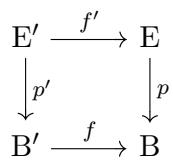
\includegraphics[keepaspectratio]{images/part001_3dd3ce93.jpg}}

一个笛卡尔方块。若 (E,p) 是局部平凡 B-纤维空间（相应地，覆叠），则 (E',p') 是以 B' 为基的局部平凡纤维空间（相应地，覆叠），且当 (E,p) 可平凡化时它亦可平凡化。

这由推论 1 得出，取其中 B = A 且 E' = B'。

推论 3. --- 设 B 为拓扑空间。设 E 与 E' 是局部平凡 B-纤维空间（相应地，覆叠）。则 \(E \times_{B} E'\) 是局部平凡 B-纤维空间（相应地，B 的覆叠）。若 E 与 E' 是可平凡化的，则它亦然。

这由推论 1 得出，取 A、B、B' 相等的情形。

命题 3. --- 设

\begin{enumerate}
\def\labelenumi{(\arabic{enumi})}
\tightlist
\item
\end{enumerate}

\pandocbounded{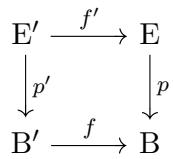
\includegraphics[keepaspectratio]{images/part001_0991252f.jpg}}

一个笛卡尔方块。假设在 B 的每一点的一个邻域内，映射 f 都有连续截面。那么，若 (E', p') 是局部平凡 B'-纤维空间（相应地，覆叠），则 B-空间 (E, p) 是局部平凡纤维空间（相应地，覆叠）。

须证 B 的每一点 \(a\) 都有邻域 U，使得 \((\mathrm{E}, p)\) 在 U 上诱导的 U-空间是局部平凡纤维空间（相应地，覆叠）。取 \(a\) 的、在其上存在连续截面 \(s\) （\(f\) 的）的一个邻域作为 U。用 \(i: \mathrm{U} \to \mathrm{B}\) 与 \(j: \overline{p}^{-1}(\mathrm{U}) \to \mathrm{E}\) 表示典范单射。由于方块 (1) 是笛卡尔的，存在唯一的连续映射 \(s^{\prime}\colon \overline{p}^{1}(\mathrm{U})\to \mathrm{E}^{\prime}\) 使得 \(f^{\prime}\circ s^{\prime} = j\) 且 \(p^{\prime}\circ s^{\prime} = s\circ p_{\mathrm{U}}\)。方块

\[
\begin{array}{c} \stackrel {{- 1}} {{p}} (\mathrm{U}) \xrightarrow {s ^ {\prime}} \mathrm{E} ^ {\prime} \\ \Biggl \downarrow p _ {\mathrm{U}} \\ \mathrm{U} \xrightarrow {s} \mathrm{B} ^ {\prime} \end{array}\tag{2}
\]

于是它是交换的，并且它与方块 (1) 的复合正是那个笛卡尔方块。

\[
\begin{array}{c} \overline {{p}} ^ {1} (\mathrm{U}) \xrightarrow {j} \mathrm{E} \\ \Biggl \downarrow p _ {\mathrm{U}} \\ \mathrm{U} \xrightarrow {i} \mathrm{B}. \end{array}
\]

由 I, p. 15 的命题 7，方块 (2) 是笛卡尔的。推论 2 使我们得以得出结论。

注意. --- 若在命题 3 中把关于映射 f 的假设减弱为只设它是普遍严格且满的，并且 \(p'\) 是覆叠，则映射 p 是平展的 (I, p. 31, prop. 8) 且是分离的 (I, p. 27, prop. 4)，但 E 不一定是 B 的覆叠。例如，可以找到拓扑空间 B、B 的局部有限闭覆盖 \((\mathrm{A}_{i})_{i\in\mathrm{I}}\) 以及一个不是覆叠的 B-空间 \((\mathrm{E},p)\)，使得对每个 \(i\in I\)，由 \(A_{i}\) 诱导的空间 \(E_{A_{i}}\) 是 \(A_{i}\) 的覆叠 (I, p. 146, exerc. 5)。但关于一个充分条件，可参见 I, p. 77 的推论 4。

\subsection{覆叠的次数}

设 B 为拓扑空间，E 为 B 的覆叠，并用 p 表示其投影。设 C 为基数 \(\operatorname{Card}(\overline{p}^{1}(b))\) （当 b 取遍 B 时）所成的集。映射 \(b \mapsto \operatorname{Card}(\overline{p}^{1}(b))\) 是 B 到 C 中的局部常值映射。若 B 非空且映射 \(b \mapsto \operatorname{Card}(\overline{p}^{1}(b))\) 是常值的，则称覆叠 E 有次数。诸基数 \(\operatorname{Card}(\overline{p}^{1}(b))\) （对 \(b \in B\)）的公共值这时称为覆叠 E 的次数，记作 \(\deg(E, p)\)，或在不致与映射 p 相混淆时，简记作 \([E:B]\) 。

若 B 非空，则以 B 为基、以 F 为纤维型的平凡覆叠有次数，等于 Card(F)。

若 B 是连通的，则函数 \(b \mapsto \text{Card}(\overline{p}^{1}(b))\) 是常值的。于是：

命题 4. --- 非空连通空间上的每个覆叠都有次数。

设 G 为拓扑空间，\((\mathrm{F}, g)\) 为 G 的覆叠，\((\mathrm{E}, f)\) 为 F 的覆叠；设这些覆叠都有次数。若 G-空间 \((\mathrm{E}, g \circ f)\) 是覆叠，则它有次数，且 \(\deg(\mathrm{E}, g \circ f) = \deg(\mathrm{F}, g) \deg(\mathrm{E}, f)\)，它也可写成

\[
[ \mathrm{E}: \mathrm{G} ] = [ \mathrm{E}: \mathrm{F} ] [ \mathrm{F}: \mathrm{G} ].
\]

事实上，若 z 是 G 的一点，则映射

\[
f _ {g (z)} ^ {- 1}: \stackrel {{- 1}} {{f}} (\stackrel {{- 1}} {{g}} (z)) \to \stackrel {{- 1}} {{g}} (z)
\]

的诸纤维都有基数 \(\deg(\mathrm{E}, f)\)，而 \(\overline{g}^1(z)\) 的基数为 \(\deg(\mathrm{F}, g)\)。于是断言由牧羊人原理 (E, III, p. 41, prop. 9) 得出。

设 B 与 B' 为拓扑空间，(E, p) 为 B 的覆叠，(E', p') 为 B' 的覆叠。设这些覆叠都有次数；则 B × B' 的覆叠 (E × E', p × p') (I, p. 71, prop. 2) 有次数，且：

\[
\deg (\mathrm{E} \times \mathrm{E} ^ {\prime}, p \times p ^ {\prime}) = \deg (\mathrm{E}, p) \deg (\mathrm{E} ^ {\prime}, p ^ {\prime}).
\]

事实上，对每个偶对 \((b,b^{\prime})\in\mathrm{B}\times\mathrm{B}^{\prime}\)，纤维 \((\mathrm{E}\times\mathrm{E}^{\prime})_{(b,b^{\prime})}\) 就是积 \(E_{b}\times E_{b^{\prime}}^{\prime}\) 。

设 B 与 B' 为拓扑空间，(E, p) 为 B 的覆叠，(E', p') 为 B' 的覆叠，并设

\[
\begin{array}{c} \mathrm{E} ^ {\prime} \xrightarrow {f ^ {\prime}} \mathrm{E} \\ \Biggl \downarrow p ^ {\prime} \\ \mathrm{B} ^ {\prime} \xrightarrow {f} \mathrm{B} \end{array}
\]

为一个笛卡尔方块。若 B′ 非空且覆叠 (E, p) 有次数，则覆叠 (E′, p′) 有次数，等于 E 的次数 (I, p. 10, cor. of prop. 4)。

\subsection{有限覆叠}

若一个覆叠的所有纤维的基数都是有限的，则称它是局部有限的。若一个覆叠的纤维的诸基数所成之集以某个有限基数为上界，则称它是有限的。

定理 1. --- 设 E、B 为拓扑空间，\(p\colon\mathrm{E}\to\mathrm{B}\) 为映射。下列条件等价：

\begin{enumerate}
\def\labelenumi{(\roman{enumi})}
\item
  赋以映射 p 的空间 E 是 B 的局部有限覆叠；
\item
  映射 p 是平展的、逆紧的且分离的；
\item
  映射 p 是连续的、开的且分离的，其纤维是有限的，且数值函数 \(b \mapsto \text{Card}(\overline{p}^{1}(b))\) 在 B 上是上半连续的 (TG, IV, p. 28)。
\end{enumerate}

在证明中将用到下面的引理：

引理. — 设 X 与 Y 为拓扑空间。映射 \(f: X \to Y\) 是闭映射，当且仅当对 Y 的每一点 y 与纤维 \(f^{-1}(y)\) 的每一邻域 W，存在 y 的邻域 V，使得 W 包含 \(f^{-1}(V)\) 。

在此陈述中，可以只考虑 \(f^{-1}(y)\) 的那些开的邻域 W。用 F 表示 W 在 X 中的补集，便可将该陈述改述如下：映射 \(f: X \to Y\) 是闭映射，当且仅当对 X 的每个闭子集 F 与 Y 的每个不属于 \(f(F)\) 的点 y，y 有与 \(f(F)\) 不相交的邻域 V。而这一断言由闭映射的定义 (TG, I, p. 30, def. 1) 立即得出。

现在来证明定理 1。三个条件中的每一个都蕴含映射 p 是连续的、开的且分离的，并且 p 的纤维是有限的。在假设 (i) 与 (iii) 之下这是显然的；在假设 (ii) 之下，p 的纤维是离散的 (I, p. 29, remark 2) 且拟紧的 (TG, I, p. 75, th. 1)，因而是有限的 (TG, I, p. 60, example 1)。

(i)⇒(ii)：只须证明 p 是逆紧的；为此，只须证明：对覆叠 (E,p) 可在其上平凡化的每个开集 U，映射 \(p_{\mathrm{U}}\colon \overline{p}^{1}(\mathrm{U})\to\mathrm{U}\) 是逆紧的 (TG, I, p. 72, prop. 3)。

由于 \(p_{U}\) 的诸纤维是有限的，这最后的断言由 TG, I, p. 77 的推论 5 得出。

(ii)⇒(iii)：设 b 为 B 的一点，并对每个 \(x \in \overline{p}^{1}(b)\)，设 \(W_{x}\) 为 x 在 E 中的开邻域，使得 \(p \mid W_{x}\) 是单射。集合 \(W = \bigcup_{x \in \overline{p}^{1}(b)} W_{x}\) 是 \(\overline{p}^{1}(b)\) 的开邻域。由于映射 p 是闭的，由上面的引理，存在 b 的开邻域 U，使得 \(\overline{p}^{1}(U) \subset W\)。对所有 \(a \in U\)，有 \(\overline{p}^{1}(a) \subset W\)；由于 p 在每个 \(W_{x}\) 上的限制是单射，由此得 \(\text{Card}(\overline{p}^{1}(a)) \leqslant \text{Card}(\overline{p}^{1}(b))\)，这就证明了映射 \(a \mapsto \text{Card}(\overline{p}^{1}(a))\) 的上半连续性。

(iii)⇒(i)：设 b 为 B 的一点。由于纤维 \(E_{b} = \overline{p}^{1}(b)\) 是有限的且映射 p 是分离的，可以对每个 \(x \in E_{b}\) 选取 x 的开邻域 \(V_{x}^{\prime}\)，使得诸 \(V_{x}^{\prime}\) 两两不相交 (I, p. 26, Remark 4)。由于映射 p 是开的且集 \(E_{b}\) 是有限的，集 \(U^{\prime} = \bigcap_{x \in E_{b}} p(V_{x}^{\prime})\) 是 b 在 B 中的开邻域。设 U 为 b 在 B 中的开邻域，含于 \(U^{\prime}\) 且使得对所有 \(a \in U\) 有 \(\text{Card}(E_{a}) \leqslant \text{Card}(E_{b})\)。对所有 \(x \in E_{b}\)，令 \(V_{x} = V_{x}^{\prime} \cap \overline{p}^{1}(U)\)。设 a 为 U 的一点；诸集 \(E_{a} \cap V_{x}\) （对 \(x \in E_{b}\)）非空且两两不相交。因而这些集中每一个都恰含一个元素，并组成 \(E_{a}\) 的一个分拆。这就证明了对每个 \(x \in E_{b}\)，映射 \(p | V_{x}\) 是单射，并且有 \(\overline{p}^{1}(U) = \bigcup_{x \in E_{b}} V_{x}\)。由于映射 p 是开的，它诱导 \(V_{x}\) 到 U 上的同胚，从而 (E, p) 是 B 的覆叠 (I, p. 70, cor. 1 of prop. 1)。

注. --- 一个连续、分离、开、逆紧且纤维有限的映射未必是覆叠。例如映射 \(x \mapsto x^{2}\) （从 R 到 \([0; +\infty[\) 的）就是这种情形。

推论 1. --- 设 E 与 B 为拓扑空间，\(p\colon\mathrm{E}\to\mathrm{B}\) 为逆紧且分离的映射。B 中使 p 在纤维 \(\mathrm{E}_{b}\) 的每一点处都是平展的那些点 b 所成的集 U 在 B 中是开的。由 (E,p) 在 U 上诱导的 U-空间是局部有限覆叠。

使映射 p 不平展的 E 的点所成的集 F 在 E 中是闭的 (I, p. 29, remark 1)。由于映射 p 是逆紧的，其像 \(p(\mathrm{F})\) 是闭的；于是 \(p(\mathrm{F})\) 的补集 U 是开的。映射 \(p_{U}\) 是分离的 (I, p. 27, prop. 4) 且逆紧的 (TG, I, p. 72, prop. 3)。按构造，映射 \(p_{\mathrm{U}}\) 是平展的；因此它满足定理 1 的条件 (ii)。

推论 2. — 设 B 为分离的拓扑空间，E 为 B-空间。设 E 是紧的且其投影 p: E → B 是平展的。则 E 是 B 的有限覆叠。

映射 \(p\) 是分离的 (I, p. 26, remark 2) 且逆紧的 (TG, I, p. 76, cor. 2)。于是由推论 1，E 是 B 的局部有限覆叠。由于 E 是紧的，\(p(\mathrm{E})\) 是 B 的拟紧子集；从 \(p(\mathrm{E})\) 到 \(\mathbb{N}\) 中的由 \(b \mapsto \operatorname{Card} \overline{p}^1(b)\) 给出的映射是局部常值的，因而有上界 (TG, IV, p. 30, corollary)。

推论 3. --- 设 B 为拓扑空间，(E,p) 与 (E',p') 为 B-空间，f: E' → E 为 B-态射。设 E' 是 B 的局部有限覆叠。

\begin{enumerate}
\def\labelenumi{\alph{enumi})}
\item
  若映射 p 是平展且分离的，则 E-空间 (E', f) 是覆叠。
\item
  若映射 f 是满的且使空间 E' 成为 E 的覆叠，则 E 是 B 的覆叠。
\end{enumerate}

在假设 \(a\) 之下，映射 \(p\) 与 \(p'\) 都是平展且分离的，且映射 \(p'\) 是逆紧的（定理 1）。于是映射 \(f\) 是平展的 (I, p. 30, cor. 1 of prop. 6)、分离的 (I, p. 25, prop. 2 b)) 且逆紧的 (I, p. 28, prop. 5)。由定理 1，\((\mathrm{E}', f)\) 是 E 的覆叠。

现在设 \(f\) 是满的，并设 \((\mathrm{E}', f)\) 是 E 的覆叠。于是它是局部有限的，故映射 \(f\) 是逆紧且满的（定理 1）。由 I, p. 25, prop. 2, c)，映射 \(p\) 是分离的，因为 \(p' = p \circ f\) 且 \(p'\) 是分离的。映射 \(p\) 是平展的 (I, p. 29, prop. 6, d))、逆紧的 (TG, I, p. 73, prop. 5, b))，且其纤维是有限的。由定理 1，B-空间 \((\mathrm{E}, p)\) 这时是 B 的覆叠。

推论 4. --- 设

\[
\begin{array}{c} \mathrm{E} ^ {\prime} \xrightarrow {f ^ {\prime}} \mathrm{E} \\ \Big \downarrow p ^ {\prime} \\ \mathrm{B} ^ {\prime} \xrightarrow {f} \mathrm{B} \end{array}
\]

为一个笛卡尔方块。设 \((\mathrm{E}^{\prime}, p^{\prime})\) 是 \(B^{\prime}\) 的局部有限覆叠，且映射 f 是普遍严格且满的。则 \((\mathrm{E}, p)\) 是 B 的局部有限覆叠。

事实上，映射 p 是平展的 (I, p. 31, prop. 8)、逆紧的 (I, p. 21, prop. 11) 且分离的 (I, p. 27, prop. 4)。

推论 5. --- 设 B 为连通的拓扑空间，(E, p) 为 B 的有限覆叠。空间 E 只有有限多个连通分支，且其中每一个都是 B 的覆叠。

若 B 是空的，结果成立；以下设 B 非空。若 X 是 E 的开闭子集，则 p 在 X 上的限制是分离的映射 (I, p. 25, prop. 2, a) 与 I, p. 26, remark 1)、平展且逆紧的 (TG, I, p. 74, corollary 1)；由定理 1，(X, p) 是 B 的局部有限覆叠。由于 B 是连通的，这个覆叠有有限次数。若 X 异于 E，则存在点 \(b \in B\) 使得 \(X_{b} \subsetneq E_{b}\)，从而 \([X:B] < [E:B]\)。由于 B 是连通的，由此得出 E 中开闭集的每个递降序列都是平稳的。

设 \(x \in E\)；于是存在含 x 的最小的开且闭的子集 X (E, III, p. 51, prop. 6)。这样的集 X 是连通的；因此它是 x 在 E 中的连通分支。这表明 E 的连通分支都是开且闭的，且其中每一个都是 B 的覆叠。由于 B 是连通的，E 的每个连通分支都与 p 的每个纤维相交；因而 E 的连通分支个数是有限的。

命题 5. — 设 B 为拓扑空间，E 与 E′ 为 B-空间，f: E′ → E 为 B-态射。设 E 是局部有限覆叠，而赋以映射 f 的空间 E′ 是局部平凡的 E-纤维空间（相应地，是覆叠）。则 E′ 是局部平凡的 B-纤维空间（相应地，是覆叠）。

用 \(p\) 与 \(p'\) 分别表示 B-空间 E 与 E' 的投影。设 \(b\) 为 B 的一点。存在 \(b\) 在 B 中的开邻域 U 以及有限分拆 \((\mathrm{V}_i)_{i\in \mathrm{I}}\) （\(\overline{p}^1 (\mathrm{U})\) 的、由 E 的开集组成的），使得对每个 \(i\in \mathrm{I}\)，映射 \(p\) 诱导 \(\mathrm{V}_i\) 到 U 上的同胚。令 \(\mathrm{V}_i' = f^{-1}(\mathrm{V}_i)\)。诸集 \(\mathrm{V}_i'\) 在 E' 中是开的，组成 \(\overline{p'}^{1}(\mathrm{U})\) 的分拆，且从 \(\mathrm{V}_i'\) 到 U 中的、由 \(p'\) 通过子空间诱导的映射使 \(V_i'\) 成为局部平凡的 U-纤维空间。由此得出，空间 \(\overline{p'}^{1}(\mathrm{U})\) 赋以映射 \(p_U': \overline{p'}^{1}(\mathrm{U}) \to U\) 后是局部平凡的 U-纤维空间 (I, p. 69, remark 2)。若 \((E', f)\) 是 E 的覆叠，则 \(p_U'\) 的纤维是离散的，因为它们与诸开集 \(V_i'\) 中每一个的交都是离散的。证明完毕。

注. --- 若 (E, p) 是 B 的覆叠且 (E', f) 是 E 的覆叠，则映射 \(p \circ f\) 是平展的 (I, p. 29, prop. 6, a)) 且分离的 (I, p. 25, prop. 2, a))。但可能发生这样的情形（见 I, p. 146 的习题 5, b)）：赋以映射 \(p \circ f\) 的空间 E′ 不是 B 的覆叠。不过参见 IV, p. 342, prop. 3。

\subsection{局部连通空间上的覆叠}

设 B 为拓扑空间，E 为 B-空间。设其投影 p 是平展且分离的映射。

若空间 B 是局部连通的，则空间 E 是局部连通的。若空间 E 是局部连通的，则 B 的开子集 \(p(\mathrm{E})\) （参看 I, p. 29, remark 2）是局部连通的。

像 \(s(\mathrm{B})\) ——这里 \(s\) 是 \(p\) 的任一截面——是开的 (I, p. 30, cor. 3) 且在 B 中是闭的 (I, p. 27, prop. 3)。若 B 是连通且非空的，则它是 E 的一个连通分支；一般地，它是 E 的若干连通分支的并。

若 B 是局部连通的，则 p 的诸截面的像的并因而是 E 的既开又闭的子集（参看 TG, I, p. 85）。

设 E 是 B 的可平凡化覆叠，\(g: E \to B \times F\) 是一个平凡化。若空间 B 是连通的，则诸集 \(V_{x} = \overline{g}^{1}(B \times \{x\})\) （当 x 取遍 F 时）就是 E 的连通分支（参看 I, p. 69 的 prop. 1）。

命题 6. --- 设 B 为拓扑空间，E 为 B-空间；用 p 表示其投影。设空间 E 是局部连通的。E 是 B 的覆叠，当且仅当 B 的每一点都有开邻域 U，使得映射 p 诱导 \(\overline{p}^{1}(U)\) 的每个连通分支到 U 上的同胚。

设 \(b\) 为 B 的一点。若 E 是 B 的覆叠，则 \(b\) 的每个连通的且使覆叠 E 在其上可平凡化的开邻域 U 都满足命题中所述的条件。反之，设 U 为满足这些条件的 \(b\) 的开邻域。集 \(\overline{p}^{1}(\mathrm{U})\) 是开的；其连通分支是 E 的开子集 (TG, I, p. 85, prop. 11) 且组成 \(\overline{p}^{1}(\mathrm{U})\) 的一个分拆。于是命题由 I, p. 70 的命题 1 的推论 1 得出。

推论 1. — 设 B 为局部连通的拓扑空间，(E,p) 为 B 的覆叠，E' 为 E 的既开又闭的子集。B-空间 (E',p \textbar{} E') 是覆叠，且 p(E') 在 B 中既开又闭。

空间 E 与 E′ 是局部连通的。对 B 的每个开子集 U，集 \(\mathrm{E}'\cap\overline{p}^{1}(\mathrm{U})\) 在 \(\overline{p}^{1}(\mathrm{U})\) 中既开又闭，因而它是 \(\overline{p}^{1}(\mathrm{U})\) 的若干连通分支的并。B 的使 p 诱导 \(\overline{p}^{1}(\mathrm{U})\) 的每个连通分支到 U 上的同胚的那些开子集 U 覆盖 B。由该命题，\(p\mid E'\) 使 \(E'\) 成为 B 的覆叠。第二个断言由此得出（参看 I, p. 68）。

推论 2. --- 设 B 为局部连通的拓扑空间，(E,p)、(E',p') 为 B 的覆叠，f,g: E' → E 为 B-态射。对 B 的每一点 b，用 \(f_b,g_b\) 表示 f 与 g 分别诱导的映射 \(\mathrm{E}_b\to \mathrm{E}_b'\) 。B 中使 \(f_b = g_b\) 的点 b 所成的集在 B 中既开又闭。

设 X 为 \(E'\) 中使 \(f(x) = g(x)\) 的点 x 所成的集。这就是 \(p'\) 到 E 中的提升 f 与 g 相重合的点所成的集；因而 X 在 \(E'\) 中既开又闭（I, p. 34 的 prop. 11）。X 的补集 Y 也是既开又闭的；于是 \(p(Y)\) 在 B 中既开又闭（推论 1）。它的补集，即 B 中使 \(f_{b} = g_{b}\) 的点 b 所成的集，因而也是既开又闭的。

推论 3. --- 设 B 为连通且局部连通的拓扑空间，(E, p) 与 (E', p') 为 B 的覆叠。对 B 的每一点 b，由 \(f \mapsto f_b\) 给出的从 \(\mathcal{C}_{\mathrm{B}}(\mathrm{E}'; \mathrm{E})\) 到 \(\mathcal{C}(\mathrm{E}_b'; \mathrm{E}_b)\) 中的映射是单射。

设 \(b\) 为 B 的一点。设 \(f\) 与 \(g\) 为从 E' 到 E 中的 B-态射，使得 \(f_b = g_b\)。B 的点 \(a\) （使 \(f_a = g_a\) 的那些）所成的集在 B 中既开又闭（推论 2）且含有 b。因而它等于 B，且 f 等于 g。

推论 4. --- 设 B 为连通且局部连通的拓扑空间，(E, p) 为 B 的覆叠，b 为 B 的一点。E 是可平凡化覆叠，当且仅当纤维 \(E_{b}\) 的每一点都属于 p 的某个连续截面的像。

该条件是必要的。设 \(E'\) 为 p 的诸连续截面的像的并，\(E''\) 为它在 E 中的补集。集 \(E'\) 在 E 中既开又闭（参看 I, p. 79）。于是 \((\mathrm{E}', p \mid \mathrm{E}')\) 是 B 的覆叠（推论 1），且由 I, p. 70 的推论 2，这个覆叠是可平凡化的。设 \(E'\) 含有 \(E_b\)，而来证明 \(E''\) 是空的。由于 \(E''\) 在 E 中既开又闭，\(p(\mathrm{E}'')\) 在 B 中既开又闭（推论 1）。由于 B 是连通的且 b 不属于 \(p(\mathrm{E}'')\)，有 \(p(\mathrm{E}'') = \varnothing\)，从而 \(E'' = \varnothing\)。

推论 5. --- 设

\pandocbounded{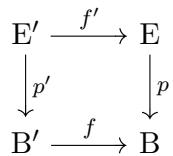
\includegraphics[keepaspectratio]{images/part001_2db9b8ac.jpg}}

为一个笛卡尔方块。设 B-空间 (E, p) 是覆叠，且空间 B' 是连通且局部连通的。设 b' 为 B' 的一点。B'-空间 (E', p') 是可平凡化覆叠，当且仅当对 E 的每个满足 \(p(x) = f(b')\) 的点 x，存在 f 的连续提升 \(g: B' \to E\)，使得 \(g(b') = x\)。

回忆 \((\mathrm{E}^{\prime}, p^{\prime})\) 是 \(B^{\prime}\) 的覆叠 (I, p. 71, cor. 2)，且映射 \(f^{\prime}\) 诱导双射 \(E_{b^{\prime}}^{\prime} \to E_{f(b^{\prime})}\) (I, p. 10, cor.)。由 I, p. 9 的 prop. 3，映射 \(s \mapsto f^{\prime} \circ s\) 定义了 \(p^{\prime}\) 的连续截面所成之集与 f 到 E 中的连续提升所成之集之间的一个双射。于是该推论由推论 4 得出。

命题 7. --- 设 B 为拓扑空间，E 与 E' 为 B-空间，f: E' → E 为 B-态射。设 E' 是 B 的覆叠且空间 B 是局部连通的。

\begin{enumerate}
\def\labelenumi{\alph{enumi})}
\item
  若 B-空间 E 的投影是平展且分离的映射，则 \((\mathrm{E}^{\prime}, f)\) 是 E 的覆叠。
\item
  若 f 是满的，则 E 是 B 的覆叠。
\end{enumerate}

用 \(p\) 与 \(p'\) 分别表示 B-空间 E 与 E′ 的投影。在假设 \(a\) 之下，\(f\) 是平展的 (I, p. 29, prop. 6, c))。在假设 \(b\) 之下，\(p\) 是平展的（同处 d)）。因此，在这两个假设的任一个之下，E 都是局部连通的；其连通分支特别在 E 中既开又闭 (TG, I, p. 85, prop. 11)。

我们先在附加假设——B 是连通且局部连通的，而 E' 是平凡覆叠 (B × F', pr₁)——之下证明命题 7。

引理. --- 若 U 是 E' 的一个连通分支，则 f 在 U 上的限制诱导 U 到 E 的某个连通分支上的同胚。

设 \(x \in F'\) 使得 \(U = B \times \{x\}\) （参看 I, p. 79）。把 \(b \in B\) 映为 \(f(b, x)\) 的从 B 到 E 中的映射是 p 的连续截面。其像 X 因而是连通的且在 E 中是开的，因为 p 是平展的 (I, p. 30, cor. 3)。而且在假设 a) 之下它还是闭的，因为 p 是分离的 (I, p. 27, prop. 3)。在假设 b) 之下它也是闭的，由 I, p. 80 的推论 1，因为 U 在 E' 中既开又闭。于是 X 是 E 的一个连通分支。

由于 \(f \mid \mathrm{U} \colon \mathrm{U} \to \mathrm{X}\) 是双射且是开的，它是到其像上的同胚，这就证明了引理。

保留引理前面的假设，现在来证明断言 \(a\) )。设 V 为 E 的一个连通分支。它是 E 中的既开又闭集，而 \(f^{-1}(\mathrm{V})\) 是 \(\mathrm{E}'\) 的若干连通分支的并，由引理，\(f\) 把这些分支同胚地映到 V 上。由 I, p. 79 的 prop. 6 得出 \((\mathrm{E}', f)\) 是覆叠。

来证明 b)。由于 f 是满的，由引理得出 E 的每个连通分支 V 都是某个连通分支 \(U = B \times \{x\}\) （\(E'\) 的）的同胚像。于是映射 p 诱导 V 到 B 上的同胚。由 prop. 6，E 是 B 的覆叠。

这就在附加假设——B 是连通的且 E' 是 B 的可平凡化覆叠——之下证明了命题。来证明一般情形。

存在 B 的由连通开集组成的覆叠 \((\mathrm{U}_{i})_{i\in\mathrm{I}}\)，覆叠 \(E'\) 在这些开集上均可平凡化。设 \(i\in I\) 。

来证明 \(a\)。若映射 \(p\) 是平展且分离的，则映射 \(p_{\mathrm{U}_i}\colon \mathrm{U}_i\times_{\mathrm{B}}\mathrm{E}\to \mathrm{U}_i\) （对 \(i\in \mathrm{I}\)）同样如此，这由 I, p. 31 的 prop. 8 与 I, p. 27 的 prop. 4 得出。于是由已处理的特殊情形得出，对每个 \(i\in \mathrm{I}\)，\(\mathrm{U}_i\)-空间 \((\overline{p'}^{1}(\mathrm{U}_i),f_{\mathrm{U}_i})\) 是覆叠。用 A 表示不交并 \(\coprod_{i\in I}\mathrm{U}_i\) 的全空间，用 \(q\colon \mathrm{A}\to \mathrm{B}\) 表示典范映射。于是，空间 \(\mathrm{A}\times_{\mathrm{B}}\mathrm{E}'\) （赋以映射 \(f_{\mathrm{A}}\colon \mathrm{A}\times_{\mathrm{B}}\mathrm{E}'\to \mathrm{A}\times_{\mathrm{B}}\mathrm{E}\) 的）是 \(\mathrm{A}\times_{\mathrm{B}}\mathrm{E}\) 的覆叠。映射 \(q\) 在 B 的每一点的邻域内都有连续截面，而把 I, p. 72 的命题 3 应用于笛卡尔方块

\[
\begin{array}{c} \mathrm {A\times_ {B} E^ {\prime}} \longrightarrow \mathrm {E^ {\prime}} \\ \Big \downarrow f _ {\mathrm{A}} \\ \mathrm {A\times_ {B} E} \longrightarrow \mathrm{E} \end{array} ,
\]

蕴含 \(E'\) 是 E 的覆叠。

来证明 \(b\)。设 \(f\) 是满的。于是对 I 的每个元素 \(i\)，映射 \(f_{\mathrm{U}_i}\colon \mathrm{U}_i\times_{\mathrm{B}}\mathrm{E}'\to \mathrm{U}_i\times_{\mathrm{B}}\mathrm{E}\) 是满的，且空间 \(\mathrm{U}_i\times_{\mathrm{B}}\mathrm{E}'\) （赋以映射 \(f_{\mathrm{U}_i}\) 的）是 \(\mathrm{U}_i\times_{\mathrm{B}}\mathrm{E}\) 的覆叠 (I, p. 71, cor. 2 of prop. 2)。由前面处理的特殊情形得出，\(\mathrm{U}_i\)-空间 \((\overline{p}^{1}(\mathrm{U}_{i}),p_{\mathrm{U}_{i}})\) 是覆叠。从而 E 是 B 的覆叠。

设 B 为拓扑空间，E 与 E′ 为 B 的覆叠，\(f: E \rightarrow E'\) 为 B-态射。我们已经看到，在下列两个假设的每一个之下，\((E, f)\) 都是覆叠：1) 覆叠 E 是局部有限次的 (I, p. 76, cor. 1)；2) 空间 B 是局部连通的 (I, p. 81, prop. 7)。这一现象可以解释如下。

设 F 与 F′ 为离散拓扑空间，\(f: B \times F \to B \times F'\) 为 B-态射。由 \(\widetilde{f}: b \mapsto \mathrm{pr}_{2} \circ f(b, \cdot)\) 给出的从 B 到空间 \(\mathcal{C}_{c}(F; F')\) 中的映射是连续的 (TG, X, p. 28, th. 3)。若 U 是 B 的开子集且映射 \(\widetilde{f}\) 在 U 上是常值的，则由 f 诱导出的映射 \(f_{U}: U \times F \to U \times F'\) 是可平凡化覆叠 (I, p. 69, prop. 1)。

空间 \(\mathcal{C}_c(\mathrm{F};\mathrm{F}')\) 无非就是映射所成之集 \(\mathcal{F}(\mathrm{F};\mathrm{F}')\) （从 F 到 \(\mathrm{F}'\) 中的），赋以经由典范同构由积空间 \((\mathrm{F}')^{\mathrm{F}}\) 的拓扑所诱导的拓扑。对这个拓扑，空间 \(\mathcal{F}(\mathrm{F};\mathrm{F}')\) 是全不连通的 (I, p. 84, prop. 10)。于是，若空间 B 是连通的，则映射 \(\widetilde{f}\) 是常值的 (I, p. 82, prop. 4)；若空间 B 是局部连通的，则映射 \(\widetilde{f}\) 是局部常值的。当集 F 有限时，空间 \(\mathcal{F}(\mathrm{F};\mathrm{F}')\) 是离散的，而映射 \(\widetilde{f}\) 是局部常值的。

注. --- 设 B 为拓扑空间，\((\mathrm{E}, p)\) 与 \((\mathrm{E}', p')\) 为 B-空间，\(f: E' \to E\) 为 B-态射。

\begin{enumerate}
\def\labelenumi{\alph{enumi})}
\item
  若 E 与 E' 是 B 的覆叠，则映射 f 是平展的 (I, p. 29, prop. 6) 且分离的 (I, p. 25, prop. 2)。但若空间 B 不是局部连通的，则一般而言 (E', f) 未必是 E 的覆叠 (I, p. 145, exerc. 4)。
\item
  若 \((\mathrm{E}^{\prime}, p^{\prime})\) 是 B 的覆叠，f 是满的且使 \(E^{\prime}\) 成为 E 的覆叠，则映射 p 是平展的 (I, p. 29, prop. 6)。但若空间 B 不是局部连通的，则一般而言它未必是分离的 (I, p. 145, exerc. 4)。特别地，E 未必是 B 的覆叠。
\end{enumerate}

推论. --- 设 B 为连通且局部连通的拓扑空间。设 E 与 E' 为 B 的覆叠。设 b 为 B 的一点。设 \(f: E' \to E\) 为 B-态射，\(f_{b}: E_{b}' \to E_{b}\) 为 f 通过限制到纤维上所诱导的映射。若映射 \(f_{b}\) 是单射（相应地，满射，相应地，双射），则映射 f 亦然。

用 \(p\) 表示 B-空间 E 的投影。由该命题，\((\mathrm{E}', f)\) 是 E 的覆叠；其像 \(f(\mathrm{E}')\) 在 E 中既开又闭。用 U 表示 \(f(\mathrm{E}')\) 在 E 中的补集，于是 B-空间 \((\mathrm{U}, p \mid \mathrm{U})\) 是 B 的覆叠 (I, p. 80, corollary 1)。若映射 \(f_b\) 是满的，则这个覆叠在 \(b\) 处的纤维是空的。由于 B 是连通空间，这时 U 是空的，故 \(f\) 是满的。

E 中使 f 的纤维恰含一个元素的点所成的集 V 是既开又闭的。B-空间 \((V, p|V)\) 与 \((f(E'), p|f(E'))\) 是 B 的覆叠（同处），且典范映射 \(i: V \to f(E')\) 是 B-态射。若映射 \(f_b\) 是单射，则映射 \(i_b\) 是满的，故由前述结果 i 是满的，从而 \(V = f(E')\)。于是映射 f 是单射。

\subsection{仿紧空间上的覆叠}

命题 8. --- 仿紧空间 (I, p. 69) 上的覆叠是仿紧空间。

先证明一个引理。

引理. --- 设 E 为分离的拓扑空间。设 E 有局部有限开覆盖 \((\mathrm{V}_{i})_{i\in\mathrm{I}}\)，使得对每个 \(i\in I\)，\(\overline{V_{i}}\) 都是仿紧空间。则空间 E 是仿紧的。

设 \((\mathrm{W}_{j})_{j\in\mathrm{J}}\) 为 E 的开覆盖；我们来证明存在 E 的局部有限开加细 \((\mathrm{A}_{k})_{k\in\mathrm{K}}\)，它比覆盖 \((\mathrm{W}_{j})_{j\in\mathrm{J}}\) 更细。对所有 \(i\in I\)，设 \((\mathrm{A}_{\ell}^{\prime})_{\ell\in\mathrm{K}_{i}}\) 为 \(\overline{V_{i}}\) 的由 \(\overline{V_{i}}\) 的开子集组成的局部有限覆盖，比覆盖 \((\mathrm{W}_{j}\cap\overline{\mathrm{V}_{i}})_{j\in\mathrm{J}}\) 更细。设 K 为族 \((\mathrm{K}_{i})_{i\in\mathrm{I}}\) 的和 (E, II, p. 30, def. 8)。对 K 的每个元素 \(k=(\ell,i)\)，令 \(A_{k}=A_{\ell}^{\prime}\cap V_{i}\)。于是 \(A_{k}\) 在 E 中是开的，且有 \(\bigcup_{k\in K}A_{k}=\bigcup_{i\in I}V_{i}=E\)；此外，对每个 \(k\in K\)，存在指标 \(j\in J\)，使得 \(A_{k}\subset W_{j}\)。于是族 \((\mathrm{A}_{k})_{k\in\mathrm{K}}\) 是 E 的比 \((\mathrm{W}_{j})_{j\in\mathrm{J}}\) 更细的开覆盖。剩下要证明族 \((\mathrm{A}_{k})_{k\in\mathrm{K}}\) 是局部有限的。设 \(x\in E\)；存在开邻域 U （x 的），它只与那些 \(V_{i}\) （其 i 属于 I 的有限子集 I'）相交。对每个 \(i\in I'\)，x 有开邻域 \(U_{i}\subset U\)，它只与有限多个开集 \(A_{k}\) （对 \(k\in K_{i}\times\{i\}\)）相交：若 x 不属于 \(\overline{V_{i}}\)，这是显然的；而若 x 属于 \(\overline{V_{i}}\)，这由覆盖 \((\mathrm{A}_{\ell}^{\prime})_{\ell\in\mathrm{K}_{i}}\) （\(\overline{V_{i}}\) 的）的局部有限性质得出。于是 \(V^{\prime}=\bigcap_{i\in I'}U_{i}\) 是 x 的开邻域，它只与诸 \(A_{k}\) （\(k\in K\)）中的有限多个相交，从而覆盖 \((\mathrm{A}_{k})_{k\in\mathrm{K}}\) 是局部有限的。

来证明该命题。设 E 为 B 的覆叠，用 p 表示其投影，并设空间 B 是仿紧的。设 \((\mathrm{A}_{i})_{i\in\mathrm{I}}\) 为 B 的局部有限开覆盖，使得对每个 \(i\in I\)，覆叠 E 在 \(A_{i}\) 上可平凡化。对所有 \(i\in I\)，设 \(F_{i}\) 为离散拓扑空间，并设 \(g_{i}\colon\overline{p}^{1}(\mathrm{A}_{i})\to\mathrm{A}_{i}\times\mathrm{F}_{i}\) 为 E 在 \(A_{i}\) 上的一个平凡化。设 \((\mathrm{B}_{i})_{i\in\mathrm{I}}\) 为 B 的开覆盖，使得对每个 \(i\in I\)，有 \(\overline{B_{i}}\subset A_{i}\) (TG, IX, p. 49, prop. 4 与 p. 48, cor. 1)。对每个 \(i\in I\)，令 \(V_{i}=\overline{p}^{1}(\mathrm{B}_{i})\)；我们有 \(\overline{V_{i}}\subset\overline{p}^{1}(\overline{\mathrm{B}_{i}})\subset\overline{p}^{1}(\mathrm{A}_{i})\) 以及 \(V_{i}=\overline{g_{i}}^{1}(\mathrm{B}_{i}\times\mathrm{F}_{i})\)，从而 \(\overline{V_{i}}\subset\overline{g_{i}}^{1}(\overline{\mathrm{B}_{i}}\times\mathrm{F}_{i})\)。由于 B 是仿紧的，\(\overline{B_{i}}\) 是仿紧的 (TG, I, p. 69, prop. 16)，且 \(\overline{B_{i}}\times F_{i}\) 是仿紧的 (TG, I, p. 70, prop. 18)。于是 \(\overline{g_{i}}^{1}(\overline{\mathrm{B}_{i}}\times\mathrm{F}_{i})\) 是仿紧的，从而 \(\overline{V_{i}}\) 也是仿紧的 (TG, I, p. 69, prop. 16)。族 \((\mathrm{V}_{i})_{i\in\mathrm{I}}\) 按构造是 E 的局部有限开覆盖。最后，空间 E 是分离的 (I, p. 26, remark 3)。因此它满足引理的假设，由此得出命题。

注. --- 可以证明，可度量化空间上的覆叠是可度量化的 (I, p. 145, exerc. 1)，而局部紧且无穷可数空间上的连通覆叠本身是局部紧且无穷可数的 (I, p. 145, exerc. 2)。

\subsection{局部常值层}

设 B 为拓扑空间，F 为一个集；给 F 赋以离散拓扑。称以 F 为茎型的 B 上常值层为 B 上以 F 为值的局部常值函数所成的层 (I, p. 45, example 2)。当不致担心与空间 B 相混淆时，这个层有时记作 \(\underline{\mathbf{F}}\)。它与平展 B-空间 \((B \times F,\mathrm{pr}_1)\) 的连续截面在 B 上所成的层相恒同：公式 \(i([U,s,a]) = (a,s(a))\) 确实定义了一个典范同构 \(i\) （从与 \(\underline{\mathbf{F}}\) 相伴的平展空间到 \((B \times F,\mathrm{pr}_1)\) 上的）。对每个 \(a \in B\)，映射 \([U,s,a] \mapsto s(a)\) 是茎 \(\underline{\mathbf{F}}_a\) （\(\underline{\mathbf{F}}\) 在 \(a\) 处的）到集 F 上的典范双射。

设 \(\mathcal{P} = (\mathcal{P}(\mathrm{U}), r_{\mathrm{UV}})\) 为 B 上的预层，使得对 B 的每个开集 U 有 \(\mathcal{P}(\mathrm{U}) = \mathrm{F}\)，且对 B 的每对开集 (U, V) 有 \(r_{\mathrm{UV}} = \mathrm{Id}_{\mathrm{F}}\) （只要 \(\mathrm{U} \subset \mathrm{V}\)）。于是，层 \(\widetilde{\mathcal{P}}\) （与 \(\mathcal{P}\) 相伴的）典范地同构于常值层 \(\underline{\mathrm{F}}\) (I, p. 52, example 1)。

定义 3. --- 拓扑空间 B 上的层 \(\mathcal{F}\) 是局部常值的，如果 B 的每一点都有开邻域 U，使得诱导层 \(\mathcal{F} \mid U\) 同构于 U 上的一个常值层。

命题 9. --- 一个层是局部常值的，当且仅当与之相伴的平展空间是覆叠。

设 B 为拓扑空间，\(\mathcal{F}\) 为 B 上的层。层 \(\mathcal{F}\) 是常值的，当且仅当平展空间 \(\mathrm{E}_{\mathcal{F}}\) B-同构于平凡覆叠 \((\mathrm{B} \times \mathrm{F},\mathrm{pr}_1)\)，其中 F 是离散拓扑空间。若 U 是 B 的开子集，则与诱导层 \(\mathcal{F} \mid \mathrm{U}\) 相伴的平展空间与 \(\mathrm{E}_{\mathcal{F}}\) 在 U 上诱导的 U-平展空间相恒同（参看 I, p. 51）。命题由此得出。

推论. --- 一个平展 B-空间是覆叠，当且仅当其截面的层是局部常值的。

这由该命题以及 I, p. 52 的例 2 得出。

\subsection{局部常值层的积}

设 B 为拓扑空间，\((\mathcal{F}_{i})_{i\in\mathrm{I}}\) 为 B 上的一个层族。用 \(\mathcal{F}\) 表示积层 \(\prod_{i\in I}\mathcal{F}_{i}\)，并对 \(i\in I\)，设 \(pr_{i}\colon \mathcal{F}\to\mathcal{F}_{i}\) 为指标 i 的投影态射 (I, p. 46, example 7)。设 \((\mathrm{E},p)\) 与 \((\mathrm{E}_{i},p_{i})\) 为分别与层 \(\mathcal{F}\) 和 \(\mathcal{F}_{i}\) 相伴的平展 B-空间，并设 \(\varphi_{i}\colon \mathrm{E}\to \mathrm{E}_{i}\) 为与 \(pr_{i}\) 相伴的 B-态射 (I, p. 50)。最后，用 \((\mathrm{E}^{\prime},p^{\prime})\) 表示 B-积 \(\prod_{B}\mathrm{E}_{i}\)。由 B-空间积的泛性质 (I, p. 5)，存在唯一的 B-态射 \(\Phi\colon \mathrm{E}\to \mathrm{E}^{\prime}\)，使得对每个 \(i\in I\)，有 \(pr_{i}\circ\Phi=\varphi_{i}\)。

命题 10. --- 若集 I 是有限的，则 B-态射 \(\Phi\) 是同构。

由 I, p. 32 的推论，B-空间 \(\mathrm{E}'\) 是平展的，于是只须证明 B-态射 \(\Phi\) 是双射 (I, p. 30, cor. 2)。对 B 的每一点 b，限制 \(\Phi_b\colon \mathrm{E}_b\to \mathrm{E}'_b\) （\(\Phi\) 在 b 处纤维上的）与从 \(\varinjlim\prod_{i\in I}\mathcal{F}_{i}(U)\) 到 \(\prod_{i\in I}\varinjlim\mathcal{F}_{i}(U)\) 的典范映射相恒同，其中 U 取遍 B 的含 b 的开子集（参看 I, p. 50）。由 E, III, p. 67 的 prop. 10，这个映射是双射。

现在考虑拓扑空间 B 上局部常值层的情形。设 \((\mathrm{F}_{i})_{i\in\mathrm{I}}\) 为一个集族，并令 \(F=\prod_{i\in I}F_{i}\) 。如下定义典范态射 \(\psi=(\psi_{\mathrm{U}})\) （从常值层 \(\underline{F}\) 到积 \(\prod_{i\in I}\underline{F}_{i}\) （诸常值层 \(\underline{F}_{i}\) 的）中的）：对 B 的每个开子集 U 与每个局部常值函数 \(f\colon U\to F\) ，令 \(\psi_{\mathrm{U}}(f)=(\mathrm{pr}_{i}\circ f)_{i\in\mathrm{I}}\) 。

命题 11. --- 若集 I 是有限的，或空间 B 是局部连通的，则典范态射 \(\psi\colon\underline{\mathbf{F}}\to\prod\underline{\mathbf{F}_{i}}\) 是同构。

设 U 为 B 的开子集。显然映射 \(\psi_{\mathrm{U}}\) 是单射。来证明它是满射。只须证明：对每个族 \((f_i)_{i\in \mathrm{I}}\) （其中 \(f_{i}\) 是从 U 到 \(\mathrm{F}_i\) 中的局部常值映射）以及 U 的每一点 \(a\)，存在 \(a\) 在 U 中的邻域 V，使得对每个 \(i\in \mathrm{I}\)，映射 \(f_{i}|\mathrm{V}\) 都是常值的。当集 I 有限时，这样一个邻域的存在性是显然的。当空间 B 局部连通时，只须取 V 为 \(a\) 在 U 中的连通邻域。这就证明了命题。

推论 1. --- 局部常值层的有限积是局部常值的。

设 \((\mathcal{F}_{i})_{i\in\mathrm{I}}\) 为 B 上的局部常值层的有限族。B 的每一点 a 都有 B 中的开邻域 U，使得对每个 \(i\in I\)，层 \(\mathcal{F}_{i}\mid U\) 同构于常值层。于是这对层 \((\prod\mathcal{F}_{i})\mid U\) 也成立，后者等于 \(\prod(\mathcal{F}_{i}\mid U)\)。

推论 2. --- 设 \((\mathcal{F}_{i})_{i\in I}\) 为 B 上的层族。设空间 B 是局部连通的，且 B 的每一点都有开邻域 U，使得对每个 \(i\in I\) ，层 \(\mathcal{F}_{i}|U\) 同构于常值层。则积层 \(\prod \mathcal{F}_{i}\) 是局部常值的。

注. --- 1) 设 \((\mathrm{E}_{i}, p_{i})_{i \in \mathrm{I}}\) 为拓扑空间 B 的覆叠族。设空间 B 是局部连通的，且存在 B 的开覆盖 \((\mathrm{U}_{j})_{j \in \mathrm{J}}\)，使得对每个 \(j \in J\) 与每个 \(i \in I\)，覆叠 \(E_{i}\) 在 \(U_{j}\) 上均可平凡化。对 \(i \in I\)，设 \(F_{i}\) 为 \(E_{i}\) 的截面的局部常值层，设 \(F\) 为积层 \(\prod_{i} F_{i}\) 。由前一个推论，F 是局部常值层，因而与之相伴的平展 B-空间 E 是覆叠 (I, p. 86, prop. 8)。对 \(i \in I\)，设 \(pr_{i}: E \to E_{i}\) 为由指标 i 的投影态射 \(F \to F_{i}\) 诱导的 B-态射。

现在考虑 B 的一个覆叠 (Y, q)，且对每个 \(i \in I\)，设 \(f_i \colon Y \to E_i\) 为 B-态射。若用 G 表示 q 的截面的局部常值层，则诸 B-态射 \(f_i\) 诱导层态射 \(\widetilde{f}_i \colon G \to F_i\) 。设 \(\widetilde{f} \colon G \to F\) 为唯一的层态射，使得 \(\widetilde{f}_i = pr_i \circ \widetilde{f}\) 对所有 \(i \in I\) 成立。于是存在唯一的 B-态射 \(f \colon Y \to E\)，使得对每个 i 有 \(f_i = pr_i \circ f\)：它就是诱导 \(\widetilde{f}\) 的那个 B-态射。

有时称 E 为族 \((\mathrm{E}_i)_{i\in \mathrm{I}}\) 的积覆叠。

\begin{enumerate}
\def\labelenumi{\arabic{enumi})}
\setcounter{enumi}{1}
\tightlist
\item
  沿用前面的记号，典范 B-态射 \(\Phi\colon\mathrm{E}\to\Pi_{\mathrm{B}}\mathrm{E}_{i}\) 是双射。事实上该问题在 B 上是局部性的，故可设对每个 \(i\in\mathrm{I}\)，B-空间 \(\mathrm{E}_{i}\) 同构于 B-空间 \((\mathrm{B}\times\mathrm{F}_{i},\mathrm{pr}_{1})\)，其中 \(\mathrm{F}_{i}\) 是离散拓扑空间，从而层 \(\mathcal{F}_{i}\) 同构于层 \(\underline{\mathrm{F}}_{i}\)。由 prop. 11，层 \(\mathcal{F}\) 与层 \(\underline{\mathrm{F}}\) 相恒同，其中 \(\mathrm{F}\) 是集 \(\prod\mathrm{F}_{i}\)，赋以离散拓扑，且映射 \(\Phi\) 与典范映射 \(B \times F \rightarrow B \times (\prod_{i} F_{i})\) 相恒同，后者是双射。
\end{enumerate}

\subsection{局部连通空间上局部常值层的态射}

设 B 为拓扑空间，\((\mathrm{E},p)\) 与 \((\mathrm{E}^{\prime},p^{\prime})\) 为 B-空间。用 \(\mathcal{M} = \underline{\mathcal{M}or_{\mathrm{B}}(\mathrm{E};\mathrm{E}^{\prime})}\) 表示从 \((\mathrm{E},p)\) 到 \((\mathrm{E}^{\prime},p^{\prime})\) 中的 B-态射在 B 上所成的层 (I, p. 45, example 4)。若 U 是 B 的开集而 b 是 U 的一点，我们用 \(\theta_{b,\mathrm{U}}\colon\mathcal{M}(\mathrm{U})\to\mathcal{C}(\mathrm{E}_{b};\mathrm{E}_{b}^{\prime})\) 表示通过过渡到 b 处的纤维而得到的典范映射。我们用 \(\theta_{b}\colon\mathcal{M}_{b}\to\mathcal{C}(\mathrm{E}_{b};\mathrm{E}_{b}^{\prime})\) 表示唯一的映射，使得对 B 的每个含 b 的开集 U，\(\theta_{b,\mathrm{U}}\) 都是 \(\theta_{b}\) 与典范映射 \(\mathcal{M}(\mathrm{U})\to\mathcal{M}_{b}\) 的复合 (E, III, p. 62)。

再设 \(\mathcal{I} = \underline{\mathcal{I}som}_{\mathrm{B}}(\mathrm{E};\mathrm{E}^{\prime})\) 为从 \((\mathrm{E},p)\) 到 \((\mathrm{E}^{\prime},p^{\prime})\) 中的 B-同构在 B 上所成的层。用 \(i\colon \mathcal{I}\to \mathcal{M}\) 表示典范态射。对每个 \(b\in \mathrm{B}\)，映射 \(\theta_{b}\circ i_{b}\) 诱导映射 \(\theta_b^\prime\) ，它把 \(\mathcal{I}_b\) 映到由 \(\mathrm{E}_b\) 到 \(\mathrm{E}_b^\prime\) 上的连续双射所成之集中。

命题 12. --- 设空间 B 是局部连通的且 B-空间 E 与 E' 是覆叠。于是层 \(\mathcal{M}or_{\mathrm{B}}(\mathrm{E};\mathrm{E}')\) 是局部常值的，且对每个 \(b\in\mathrm{B}\)，映射 \(\theta_{b}\) 是从其在 \(b\) 处的茎到从 \(\mathrm{E}_{b}\) 到 \(\mathrm{E}_{b}^{\prime}\) 中的映射所成之集上的双射。

类似地，层 \(\mathcal{I}\text{som}_{\mathrm{B}}(\mathrm{E};\mathrm{E}^{\prime})\) 是局部常值的，且对 B 的每一点 \(b\)，映射 \(\theta_{b}^{\prime}\) 是从其在 \(b\) 处的茎到从 \(\mathrm{E}_{b}\) 到 \(\mathrm{E}_{b}^{\prime}\) 上的双射所成之集上的双射。

我们将用 \(\mathcal{M} = \underline{\mathcal{M}or}_{\mathrm{B}}(\mathrm{E};\mathrm{E}^{\prime})\) 与 \(\mathcal{I} = \underline{\mathcal{Isom}}_{\mathrm{B}}(\mathrm{E};\mathrm{E}^{\prime})\) 表示。要证的断言在 B 上是局部性的；因此可设 \(\mathrm{E} = \mathrm{B}\times \mathrm{F}\) 与 \(\mathrm{E}' = \mathrm{B}\times \mathrm{F}'\) 是平凡覆叠，其中 F 与 \(\mathrm{F}'\) 是离散拓扑空间。

首先来证明，对 B 的每个连通开子集 U 与 U 的每一点 b，映射 \(\theta_{b,U}\) 是双射。设 \(f\colon U\times F\to U\times F'\) 为 U-空间的态射；于是 \(\theta_{b,U}(f)\) 是映射 \(y\mapsto\mathrm{pr}_{2}(f(b,y))\) （从 F 到 \(F'\) 中的）。对所有 \(y\in F\)，映射 \(x\mapsto\mathrm{pr}_{2}(f(x,y))\) 是从连通空间 U 到离散空间 \(F'\) 中的连续映射，故为常值的，等于 \(\mathrm{pr}_{2}(f(b,y))\)。于是有 \(f(x,y)=(x,\theta_{b,U}(f)(y))\)。由此得出 \(\theta_{b,U}\) 是双射；

其逆双射把每个映射 \(\varphi\colon\mathrm{F}\to\mathrm{F}^{\prime}\) 对应到从 \(\mathrm{U}\times\mathrm{F}\) 到 \(\mathrm{U}\times\mathrm{F}^{\prime}\) 中的、由 \((x,y)\mapsto(x,\varphi(y))\) 给出的 U-态射。

按假设，每点 \(b \in B\) 都有由连通开邻域组成的基本邻域系；于是映射 \(\theta_{b}\) 是双射。诸映射 \(\theta_{b,\mathrm{U}}^{-1}\) （其中 U 取 B 的非空连通开子集而 b 取 B 的任意点）定义了从以 \(F^{\prime F}\) 为茎型的常值层到层 \(\mathcal{M}\) 的一个预层态射（关于 B 的连通开子集组成的基）。由前所证，这个态射诱导茎上的双射；因而它是同构。

关于层 \(\mathcal{I}\) 的断言类似地证明。

推论 1. --- 设 B 为拓扑空间，A 为 B 的子空间。设空间 A 与 B 都是局部连通的。设 E 与 E' 为 B 的覆叠。则典范态射 \(\psi\colon\mathcal{M}or_{B}(E;E')_{A}\to\mathcal{M}or_{A}(E_{A};E'_{A})\) 与 \(\psi'\colon\mathcal{I}som_{B}(E;E')_{A}\to\mathcal{I}som_{A}(E_{A};E'_{A})\) (I, p. 45, example 4) 都是同构。

对每点 \(a \in \mathrm{A}\)，由前一个命题以及 I, p. 63 的例 2（应用于空间 \(\{a\}\)、A、B 及典范单射）得出，典范态射 \(\psi\) 通过过渡到茎诱导 \(\mathrm{E}_a^{\mathrm{E}_a'}\) 上的恒同映射。因而它是同构。\(\psi'\) 是同构这一事实类似地证明。

推论 2. --- 设 B 为拓扑空间，A 为 B 的子空间。设空间 A 与 B 都是局部连通的，且偶对 (B, A) 满足 I, p. 37 的性质 (PCV)。设 E 与 E' 为 B 的覆叠，用 p 与 p' 表示它们的投影。设 \(g: \overline{p}^{1}(A) \to (\overline{p}')^{1}(A)\) 为 A-态射（相应地，A-同构）。则存在 A 在 B 中的邻域 U 以及 U-态射（相应地，U-同构）\(f: \overline{p}^{1}(U) \to (\overline{p}')^{1}(U)\)，使得 \(f_{A} = g\)。

保留推论 1 的记号。由同一推论，A-态射 \(g \colon \mathrm{E}_{\mathrm{A}} \to \mathrm{E}_{\mathrm{A}}^{\prime}\) 与截面 \(s_0\) （平展空间 \(\mathrm{E}_{\mathcal{M}}\) （与 \(\mathcal{M}\) 相伴的）在 A 上的）相恒同。由对偶对 (B, A) 所作的假设以及 I, p. 39 的引理 3，存在 A 在 B 中的开邻域 U 以及连续截面 \(s\) （\(\mathrm{E}_{\mathcal{M}}\) 在 U 上的、延拓 \(s_0\) 的）。这个截面 \(s\) 与一个 U-态射 \(f \colon \mathrm{E}_{\mathrm{U}} \to \mathrm{E}_{\mathrm{U}}^{\prime}\) （延拓 \(g\) 的）相恒同。

g 是 A-同构的情形类似处理，只需把层 M 换成层 S。

\section{主覆叠}

\subsection{主纤维丛}

定义 1. --- 设 G 为拓扑群，B 为拓扑空间。以 B 为基、以 G 为群的（右）主纤维丛是指赋以 G 在 E 上的右作用 (A, I, p. 50) 且满足下列性质的 B-空间 (E, p)：

(FP) 对每一点 \(b\) （\(B\) 的），存在邻域 \(U\) （\(b\) 的）以及 U-同构 \(f\colon U\times G\to \overline{p}^{1}(U)\)，使得对所有 \(u\in U\) 与 \(g,g'\in G\)，有 \(f(u,gg')=f(u,g)\cdot g'\)。

我们有时不说 \((E, p)\) 是以 B 为基、以 G 为群的主纤维丛，而说四元组 \((E, G, B, p)\) 是一个主纤维化（参看 VAR, R, §6），或者滥用术语，说映射 \(p: E \to B\) 是以 B 为基、以 G 为群的主纤维化。

当基 B、群 G 以及 G 在 E 上的作用都确定无疑时，我们就简单地说 \((E, p)\) 是主纤维丛。

设 G 为拓扑群。设 \((E,p)\) 为赋以 G 的左作用的 B-空间。若对于与给定运算相反的群 \(G^{\circ}\) 的右作用 (A, I, p. 50)，\((E,p)\) 是以 \(G^{\circ}\) 为群的主右纤维丛，则称 \((E,p)\) 是以 G 为群的主左纤维丛。

主纤维丛是局部平凡的纤维丛 (I, p. 68, def. 1)。

由性质 (FP) 得出，群 G 连续地 (TG, III, p. 9) 且自由地作用在 E 上，且这个作用的轨道就是 B-空间 (E, p) 的纤维。映射 \(p' \colon \mathrm{E} / \mathrm{G} \to \mathrm{B}\) （由 \(p\) 导出的）是连续的双射。同样由性质 (FP)，映射 \(p\) 是开的 (TG, I, p. 30, prop. 2 与 p. 26, prop. 5)；于是 \(p'\) 是同胚 (TG, I, p. 32, prop. 3)。

设 \((\mathrm{E},p)\) 与 \((\mathrm{E}^{\prime},p^{\prime})\) 为以 B 为基、以 G 为群的主纤维丛。我们称映射 \(f: E \to E^{\prime}\) 为（以 B 为基、以 G 为群的）主纤维丛的态射，如果 f 是 B-态射，且有 \(f(x \cdot g) = f(x) \cdot g\) （对所有 \(x \in E\) 与每个 \(g \in G\)）。设 \((\mathrm{E}^{\prime\prime},p^{\prime\prime})\) 为以 B 为基、以 G 为群的主纤维丛。若 \(f: \mathrm{E} \to \mathrm{E}'\) 与 \(g: \mathrm{E}' \to \mathrm{E}''\) 都是主纤维丛的态射，则映射 \(g \circ f: \mathrm{E} \to \mathrm{E}''\) 是主纤维丛的态射。按照一般定义 (E, IV, p. 11)，可以把上面定义的那些取作以 B 为基、以 G 为群的主纤维丛结构的态射。我们用 \(\mathcal{C}_{\mathrm{B}}^{\mathrm{G}}(\mathrm{E}; \mathrm{E}')\) 表示从 \((\mathrm{E}, p)\) 到 \((\mathrm{E}',p')\) 中的主纤维丛态射所成之集。

我们称以 B 为基、以 G 为群的平凡主纤维丛为 B-空间 \((B \times G, pr_{1})\) （赋以 G 在 \(B \times G\) 上的由 \((b, g) \cdot h = (b, gh)\) 定义的右作用）。

以 B 为基、以 G 为群的主纤维丛 (E, p) 称为可平凡化的，如果存在从 (E, p) 到平凡主纤维丛 \((B \times G,\mathrm{pr}_{1})\) 上的同构；这样的同构称为主纤维丛 (E, p) 的平凡化。性质 (FP) 表达的是：存在 B 的开覆盖 \((\mathrm{U}_{i})_{i \in \mathrm{I}}\)，使得对每个 \(i \in I\)，赋以由 G 在 E 上的作用所诱导的 G 的右作用的 \(\mathrm{U}_{i}\)-空间 \((\overline{p}^{1}(\mathrm{U}_{i}), p \mid \mathrm{U}_{i})\) 都是可平凡化的主纤维丛。

例. --- 1) 设 (E, p) 为以 B 为基、以 G 为群的主纤维丛，A 为 B 的子空间。E 的子空间 \(E_{A} = \overline{p}^{1}(A)\) 在 G 的作用下稳定，且映射 \(p_{A}: E_{A} \to A\) 使它成为以 A 为基、以 G 为群的主纤维丛。称 \((E_{A}, p_{A})\) 为由 (E, p) 在 A 上诱导的主纤维丛。

\begin{enumerate}
\def\labelenumi{\arabic{enumi})}
\setcounter{enumi}{1}
\tightlist
\item
  设 (E, p) 为以 B 为基、以 G 为群的主纤维丛；设 \((\mathrm{E}^{\prime}, p^{\prime})\) 为以 \(B^{\prime}\) 为基、以 \(G^{\prime}\) 为群的主纤维丛。于是便定义了群 \(G \times G^{\prime}\) 在空间 \(E \times E^{\prime}\) 上的一个右作用，其法则是令 \((x, x^{\prime}) \cdot (g, g^{\prime}) = (x \cdot g, x^{\prime} \cdot g^{\prime})\) （对 \(x \in E\)、\(x^{\prime} \in E^{\prime}\)、\(g \in G\) 与 \(g^{\prime} \in G^{\prime}\)）；这个作用是连续的。设 U 为 B 的开子集，\(f: U \times G \to \overline{p}^{1}(U)\) 为 U-空间 \((\overline{p}^{1}(U), p_{\mathrm{U}})\) 的一个平凡化；设 \(U^{\prime}\) 为 \(B^{\prime}\) 的开子集，\(f^{\prime}: U^{\prime} \times G^{\prime} \to \overline{p'}^{1}(U^{\prime})\) 为 \(U^{\prime}\)-空间 \((\overline{p'}^{1}(U^{\prime}), p_{\mathrm{U}}^{\prime})\) 的一个平凡化。映射 \(((b, b^{\prime}), (g, g^{\prime})) \mapsto (f(b, g), f'(b', g'))\) 是 \((\mathrm{U} \times \mathrm{U}^{\prime})\)-同构 \(f''\) （从 \((\mathrm{U} \times \mathrm{U}^{\prime}) \times (\mathrm{G} \times \mathrm{G}^{\prime})\) 到 \(\overline{p}^{1}(U) \times \overline{p'}^{1}(U^{\prime})\) 上的），且有
\end{enumerate}

\[
f ^ {\prime \prime} ((b, b ^ {\prime}), (g h, g ^ {\prime} h ^ {\prime})) = (f (b, g h), f ^ {\prime} (b ^ {\prime}, g ^ {\prime} h ^ {\prime})) = f ^ {\prime \prime} ((b, b ^ {\prime}), (g, g ^ {\prime})) \cdot (h, h ^ {\prime}).
\]

由此得出，\((\mathrm{B} \times \mathrm{B}')\)-空间 \(E \times E'\) （赋以上面定义的 \(G \times G'\) 的作用）是主纤维丛，称为主纤维丛 E 与 E' 的积。

\begin{enumerate}
\def\labelenumi{\arabic{enumi})}
\setcounter{enumi}{2}
\item
  特别地，当 \(B = B'\) 时，B-空间 \(E \times_{B} E'\) 与以 \(G \times G'\) 为群的、由 \(E \times E'\) 在对角线 \(\Delta_{B}\) （\(B \times B\) 的）上诱导的主纤维丛相恒同。赋以这个主纤维丛结构后，B-空间 \(E \times_{B} E'\) 称为主纤维丛 E 与 \(E'\) 的纤维积。
\item
  设 E 为以 B 为基、以 G 为群的主纤维丛，F 为拓扑空间。\((B \times F)\)-空间 \(E \times F\) （赋以作用 \((x, y) \cdot g = (x \cdot g, y)\) ，对 \(x \in E\) 、\(y \in F\) 与 \(g \in G\) ）是以 G 为群的主纤维丛。这是例 2 的特殊情形，其中 \(p'\) 是 F 的恒同映射，而 \(G'\) 是化为单位元的群。
\item
  设 B 为拓扑空间，(E, p) 为以 B 为基、以 G 为群的主纤维丛。设 B' 为拓扑空间，\(f: B' \to B\) 为连续映射。群 G 右作用于纤维积 \(B' \times_{B} E\)，其法则为 \((b', x) \cdot g = (b', x \cdot g)\) （对 \(b' \in B'\) 、\(x \in E\) 与 \(g \in G\) ）。这个作用是连续且自由的；其轨道是映射 \(pr_{1}: B' \times_{B} E \to B'\) 的纤维。由上面的例 1 与例 4 以及 I, p. 16 的注 2 得出，\(B'\)-空间 \(B' \times_{B} E\) 是以 G 为群的主纤维丛。称它为由 (E, p) 通过换基 f 导出的主纤维丛，或 (E, p) 在 f 下的逆像。
\end{enumerate}

命题 1. --- 主纤维丛的每个态射都是同构。

设 \(f \colon \mathrm{B} \times \mathrm{G} \to \mathrm{B} \times \mathrm{G}\) 为平凡主纤维丛 \((\mathrm{B} \times \mathrm{G},\mathrm{pr}_1)\) 到其自身的态射，并设 \(\varphi \colon \mathrm{B} \times \mathrm{G} \to \mathrm{G}\) 为连续映射 \(\mathrm{pr}_2 \circ f\)，使得 \(f(b, g) = (b, \varphi(b, g))\)。对所有 \(b \in \mathrm{B}\) 与所有 \(g, h \in \mathrm{G}\)，我们有 \(\varphi(b, gh) = \varphi(b, g) \cdot h\)，从而 \(\varphi(b, g) = \varphi(b, e) \cdot g\)，其中 \(e\) 表示 \(\mathrm{G}\) 的单位元。于是态射 \(f\) 是同构，其逆态射 \(f^{-1}\) 由 \(f^{-1}(b, g) = (b, \varphi(b, e)^{-1}g)\) （对 \((b, g) \in \mathrm{B} \times \mathrm{G}\) ）定义。

现在设 E 与 \(E'\) 为主纤维丛，\(f: E \to E'\) 为主纤维丛的态射。鉴于性质 (FP)，对每点 \(b \in B\) 存在 b 的开邻域 U，使得主丛 \(E_{U}\) 与 \(E'_{U}\) 都可平凡化。

通过过渡到子空间，\(f\) 诱导主纤维丛的态射 \(f_{\mathrm{U}}: \mathrm{E}_{\mathrm{U}} \to \mathrm{E}_{\mathrm{U}}'\)；据前所述，这个态射 \(f_{\mathrm{U}}\) 是同构。特别地，\(f_{b}: \mathrm{E}_{b} \to \mathrm{E}_{b}'\) 是双射。于是存在唯一的映射 \(g: \mathrm{E}' \to \mathrm{E}\)，它通过过渡到子空间诱导双射 \(f_{b}^{-1}\)。由 I, p. 19 的命题 4，映射 \(g\) 是连续的；因此 \(f\) 是主纤维丛的同构。

推论. --- 设 G 为拓扑群，\((E, p)\) 与 \((E', p')\) 为分别以 B 与 B' 为基、以 G 为群的主纤维丛。设 \(f: B' \to B\) 与 \(f': E' \to E\) 为连续映射，使得 \(p \circ f' = f \circ p'\)，且使得对每个 \(x' \in E'\) 与每个 \(g \in G\)，有 \(f'(x' \cdot g) = f'(x') \cdot g\)。则方块

\pandocbounded{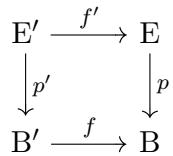
\includegraphics[keepaspectratio]{images/part001_eb35a58e.jpg}}

是一个笛卡尔方块。

事实上，映射 \(h: E' \to B' \times_{B} E\) （由 \(h(x') = (p'(x'), f'(x'))\) 定义的）是主纤维丛的 \(B'\)-态射，因而是同构；此外，我们有 \(pr_{2} \circ h = f'\)，由此得结果 (I, p. 8, prop. 2)。

在前一推论的假设下，有时称 \(f'\) 为主纤维丛的 f-态射。

命题 2. --- 设 (E, p) 为以 B 为基、以 G 为群的主纤维丛，设 \(\varepsilon\) 为截面 \(b \mapsto (b, e)\) （平凡主纤维丛 (B \(\times\) G, \(\mathrm{pr}_{1}\)) 的），其中 \(e\) 表示 G 的单位元。映射 \(h \mapsto h \circ \varepsilon\) 是从 \(\mathcal{C}_{\mathrm{B}}^{\mathrm{G}}(\mathrm{B} \times \mathrm{G}; \mathrm{E})\) 到连续截面所成之集 \(\mathcal{S}(\mathrm{B}; \mathrm{E})\) （\(p\) 的）上的双射。其逆双射把连续截面 \(s\) （\(p\) 的）对应到 B-态射 \((b, g) \mapsto s(b) \cdot g\)。

推论. --- 主纤维丛可平凡化，当且仅当它有连续截面。

命题 3. --- 设 E 与 B 为拓扑空间，\(p\colon\mathrm{E}\to\mathrm{B}\) 为连续映射，G 为右作用于 E 上的拓扑群。下列条件等价：

\begin{enumerate}
\def\labelenumi{(\roman{enumi})}
\item
  赋以映射 p 的 E 是以 B 为基、以 G 为群的主纤维丛；
\item
  对每个 \(x \in E\) 与每个 \(g \in G\) ，有 \(p(x \cdot g) = p(x)\) ，映射 \(\theta: (x, g) \mapsto (x, x \cdot g)\) 是 \(E \times G\) 到 \(E \times_{B} E\) 上的同胚，且 B 的每一点都有邻域，映射 p 在其上存在连续截面。
\end{enumerate}

(i)⇒(ii)：设 (E, p) 是主纤维丛。群 G 连续且自由地作用于 E，其轨道即 p 的纤维。于是映射 \(\theta\) 是双射且连续。更精确地说，若给 \(E \times_{B} E\) 赋以由 \((x, y) \cdot g = (x, y \cdot g)\) 定义的 G 的作用，则映射 \(\theta\) 是平凡主纤维丛 \(E \times G\) 到主纤维丛 \((E \times_{B} E \to E, \mathrm{pr}_{1})\) （例 5）中的 E-态射，因而是同构（命题 1）。(ii) 的其余断言由定义立即得出。

(ii)⇒(i)：令 \(\varphi = pr_{2} \circ \theta^{-1}\) ，于是对每个 \((x, y) \in E \times_{B} E\) ，有

\[
\theta^ {- 1} (x, y) = (x, \varphi (x, y)).\tag{1}
\]

映射 \(\varphi\colon\mathrm{E}\times_{\mathrm{B}}\mathrm{E}\to\mathrm{G}\) 是连续的，且对 \((x,y)\in\mathrm{E}\times_{\mathrm{B}}\mathrm{E}\)，元素 \(\varphi(x,y)\) 是 G 的唯一元素 \(g\) （使得 \(y=x\cdot g\) 的）。设 \(b\) 为 B 的一点；设 U 为 \(b\) 的邻域，\(s\) 为 \(p\) 在 U 上的连续截面。对 \((u,g)\in\mathrm{U}\times\mathrm{G}\)，令 \(f(u,g)=s(u)\cdot g\)；映射 \(f\) 是从 \(U \times G\) 到 \(\overline{p}^{-1}(\mathrm{U})\) 中的 U-态射。对 \(y\in\overline{p}^{-1}(\mathrm{U})\)，令 \(f'(y)=(p(y),\varphi(s(p(y)),y))\)。映射 \(f'\) 是从 \(\overline{p}^{-1}(\mathrm{U})\) 到 U \(\times\) G 中的 U-态射。我们有

\[
(f \circ f ^ {\prime}) (y) = s (p (y)) \cdot \varphi (s (p (y)), y) = y.
\]

另一方面，对 \((u,g)\in \mathrm{U}\times \mathrm{G}\) ，有

\[
(f ^ {\prime} \circ f) (u, g) = f ^ {\prime} (s (u) \cdot g) = (u, \varphi (s (u), s (u) \cdot g)) = (u, g).
\]

因此 f 是 U-同构。由此得出 \((E,p)\) 是以 B 为基、以 G 为群的主纤维丛。

注 1. --- 设 (E, p) 为以 B 为基、以 G 为群的主纤维丛。用命题 3 的记号，映射 \(\theta^{-1}\colon E \times_{B} E \to E \times G\) 是主纤维丛 \(\mathrm{pr}_{1}\colon E \times_{B} E \to E\) 的一个平凡化。称 \(\theta^{-1}\) 为这个主纤维丛的典范平凡化。

推论 1. --- 设 G 为连续右作用于拓扑空间 E 上的拓扑群。下列条件等价：

\begin{enumerate}
\def\labelenumi{(\roman{enumi})}
\item
  轨道空间 E/G 是 Hausdorff 的，且赋以典范映射 \(p: E \rightarrow E/G\) 的空间 E 是以 G 为群的主纤维丛；
\item
  群 G 逆紧地 (TG, III, p. 27) 且自由地作用于 E，且 E/G 的每一点都有邻域，映射 p 在其上存在连续截面。
\end{enumerate}

令 \(B=E/G\)。在假设 (i) 与 (ii) 的每一个之下，群 G 都连续且自由地作用于 E，于是映射 \(\theta\colon(x,g)\mapsto(x,x\cdot g)\) 是从 \(E\times G\) 到 \(E\times_{B}E\) 上的连续双射。我们置于这个假设之下，并用 \(\varphi\colon E\times_{B}E\to G\) 表示映射 \(pr_{2}\circ\theta^{-1}\)。顾及公式 (1)，\(\theta\) 是同胚，当且仅当映射 \(\varphi\) 是连续的。另一方面，由于 G 所定义的等价关系是开的 (TG, III, p. 10, lemma 2)，空间 E/G 是 Hausdorff 的，当且仅当这个等价关系的图 \(E\times_{B}E\) 在 \(E\times E\) 中是闭的。G 逆紧地作用于 E，当且仅当 \(E\times_{B}E\) 在 \(E\times E\) 中是闭的且映射 \(\varphi\) 是连续的。于是条件 (i) 与 (ii) 的等价性由命题 3 得出。

推论 2. --- 设 G 为拓扑群，H 为 G 的子群，p: G → G/H 为典范映射。若映射 p 在 G/H 的某个非空开集上有连续截面，则 p 使 G 成为以 G/H 为基、以 H 为群的主纤维丛。

通过左平移，G/H 的每一点都有邻域，映射 p 在其上有连续截面。另一方面，对 \((g,g')\) （属于 \(G\times G\) 的），令 \(\varphi(g,g')=g^{-1}g'\)。若 \(p(g)=p(g')\)，则 \(\varphi(g,g')\) 属于 H。映射 \((g,g')\mapsto(g,\varphi(g,g'))\) （从 \(G\times_{G/H}G\) 到 \(G\times H\) 的）是连续的，且是连续映射 \(\theta: G\times H\to G\times_{G/H}G\) （由 \(\theta(g,h)=(g,gh)\) 定义的）的逆，由此得该推论。

注 2. --- 这种情形特别出现于：G 是实李群，有限维、无穷可数，解析地且可迁地作用于解析流形 X。若取 H 为 X 的某点的稳定子，则映射 p 是 G 到齐性李空间 G/H 上的浸没，后者同构于 X (LIE, III, p. 109, corollary)。因此它有局部截面 (VAR, p. 50)。
